% !TEX encoding = UTF-8
% !TEX TS-program = pdflatex
% !TEX root = ../nt.tex
% !TEX spellcheck = it-IT

%************************************************
\chapter{Affidabilità e Disponibilità}
\label{cap:relavl}
%************************************************\\

\section{Starting Point}

\subsection{Exercise}

CSP = \textit{Content Service Provider}. Abbiamo una batteria di $K$ server, tutti equivalenti. Server soggetti a guasti. $M$ server di backup. Quando un server si blocca viene sostituito con un server di backup, SE DISPONIBILE. Se i $K$ server funzionano tutti siamo in "\textit{Normal State}", Se inferiori a $K$ il sistema si blocca e siamo in "\textit{Failure State}". Ce ne devono essere almeno $K$.

\{TTF per il processo expneg. con parametro $f_p$, TTF memoria expneg. con parametro $f_m$, TTF disco expneg. con parametro $f_d$\}.

DTT, probabilità di regime, frazione di tempo Failure State, MTTF del sistema; durata media dell'intervallo di tempo tra un istante in cui il servizio è attivato e l'istante successivo corrispondente alla sospensione del servizio.

In totale ci sono $\underline{K+M}$ server (server attivi + server di backup). La situazione normale sarebbe il seguente tableau: $\{K,0,M\}$, ove i tre parametri indicano rispettivamente i server funzionanti della server farm, quelli in riparazione e quelli di backup. Ad un certo punto potrebbe accadere che nella server farm vi siano $K$ server ed $M$ in riparazione. Un ulteriore guasto della server farm porterebbe il sistema ad entrare in Failure State. Dinamica relativa al sistema. Definizione di Stato: processo stocastico: numero di server nella server farm e nei server di backup. Questa definizione di stato ci va bene per un processo Markoviano. Le tre v.a. sono indipendenti. Il tempo di guasto di un server sarà il minimo di queste tre v.a. dei TTF. Se quindi $f=f_p+f_m+f_d$, allora il tempo di guasto del server sarà tale che $TTF \sim EXP(f)$. I tempi di guasto dei vari server sono v.a. indipendenti. Le riparazioni procedono in parallelo tra di loro. Tempi di riparazione indipendenti dai tempi di guasto $\iff$ PROCESSO MARKOVIANO, il cui DTT è il seguente:

\begin{center}
\begin{tikzpicture}[->, >=stealth', auto, semithick, node distance=2cm]
\tikzstyle{every state}=[fill=white,draw=black,thick,text=black,scale=1]
\node[state]    (KPM)                     {$K+M$};
\node[state]    (KPMM1)[right of=KPM]   {$K+M-1$};
\node[state]    (KPMM2)[right of=KPMM1]   {$K+M-2$};
\node[state] (KPMM3) [right of=KPMM2] {$K+M-3$};
\node[state]    (d)[right of=KPMM3]   {\ldots};
\node[state]    (KP1)[right of=d]   {$K+1$};
\node[state]    (K)[right of=KP1]   {$K$};
\node[state]    (KM1)[right of=K]  {$K-1$};
\path
(KPM) edge[bend left]     node{$Kf$}         (KPMM1)
(KPMM1) edge[bend left]     node{$Kf$}         (KPMM2)
    edge[bend left,below]    node{$\mu$}            (KPM)
(KPMM2) edge[bend left]     node{$Kf$}           (KPMM3)
    edge[bend left,below]    node{$2\mu$}             (KPMM1)
(KPMM3) edge[bend left]         node{$Kf$}   (d)
	edge[bend left,below]   node{$3\mu$}          (KPMM2)
(d) edge[bend left]       node{$Kf$}  (KP1)
	  edge[bend left,below]   node{$4\mu$}     (KPMM3)
(KP1)   edge[bend left]   node{$Kf$}      (K)
      edge[bend left,below]  node{$(M-1)\mu$}          (d)
(K) edge[bend left]       node{$Kf$}  (KM1)
	 edge[bend left,below]   node{$M\mu$}      (KP1)
(KM1) edge[bend left,below]   node{$(M+1)\mu$}     (K);
\end{tikzpicture}
\end{center}

Il numero di stati è finito $(\iff \cardinality{stati}<+\infty)$. Si suppone che le riparazioni avvengano in parallelo, altrimenti se ci fosse una Single Repair Facility $\mu$ sarebbe costante. Quindi abbiamo: $N(t)=K+M$, ovvero $K$ server nella server farm che si possono guastare. Il tempo di guasto è dato da $\rightarrow$

\[
	\phi_{K+M}(t) = \underline{\min{(\dots)}}
\]

ove la parte sottolineata indica i tempi di guasto residui al tempo $t$. Se siamo nello stato $K$, vi sono $M$ \underline{in riparazione} e 0 nella stanza dei server di backup. Può accadere che ad un certo punto si guasti un ulteriore server della server farm $\implies$ FAILURE STATE. La velocità totale di uscita dallo stato $K+M$ sarebbe proprio $Kf$.

\begin{itemize}

\item{\textbf{NORMAL STATE}} fino a $K$;
\item{\textbf{FAILURE STATE}} $K-1$;
\end{itemize}

Oscillazione tra normal state e failure state. La seguente Catena di Markov vagherà tra questi stati. Non esiste una singola definizione di stato. Ce ne possono essere differenti. Alcune volte delle differenti definizioni di stato potrebbero portare allo stesso DTT. Considerando ad esempio $N(t)$ come il numero di server in riparazione avremo il seguente DTT:

\begin{center}
\begin{tikzpicture}[->, >=stealth', auto, semithick, node distance=2cm]
\tikzstyle{every state}=[fill=white,draw=black,thick,text=black,scale=1]
\node[state]    (0)                     {$0$};
\node[state]    (1)[right of=0]   {$1$};
\node[state]    (2)[right of=1]   {$2$};
\node[state] (3) [right of=2] {$3$};
\node[state]    (d)[right of=3]   {\ldots};
\node[state]    (MM1)[right of=d]   {$M-1$};
\node[state]    (M)[right of=MM1]   {$M$};
\node[state]    (MP1)[right of=M]  {$M+1$};
\path
(0) edge[bend left]     node{$Kf$}         (1)
(1) edge[bend left]     node{$Kf$}         (2)
    edge[bend left,below]    node{$\mu$}            (0)
(2) edge[bend left]     node{$Kf$}           (3)
    edge[bend left,below]    node{$2\mu$}             (1)
(3) edge[bend left]         node{$Kf$}   (d)
	edge[bend left,below]   node{$3\mu$}          (2)
(d) edge[bend left]       node{$Kf$}  (MM1)
	  edge[bend left,below]   node{$4\mu$}     (3)
(MM1)   edge[bend left]   node{$Kf$}      (M)
      edge[bend left,below]  node{$(M-1)\mu$}          (d)
(M) edge[bend left]       node{$Kf$}  (MP1)
	 edge[bend left,below]   node{$M\mu$}      (MM1)
(MP1) edge[bend left,below]   node{$(M+1)\mu$}     (M);
\end{tikzpicture}
\end{center}


ove cambierebbero solo le label rispetto al precedente.
Non è importante il modo in cui si chiamino gli stati, ma le loro transizioni! PROCESSO STOCASTICO: numero di server in riparazione al tempo $t$; CATENA ERGODICA (OMOGENEA, IRRIDUCIBILE con $\cardinality{stati}<+\infty$). In funzione della distribuzione di regime dobbiamo trovare altre quantità:

$\pi_{M+1}$ sarebbe la frazione di tempo a regime ove il servizio è sospeso, quindi $\underline{1-\pi_{M+1}} = \underline{\pi_0+\ \dots+\ \pi_M}$ sarebbe invece la frazione di tempo a regime nel quale il sistema si trova nello stato NORMAL, per via della condizione di NORMALIZZAZIONE. Il LHS è proprio la DISPONIBILIT\`A.

$\underline{1-\pi_{M+1}}$ AVAILABILITY del mio sistema di servizio. MTTF: durata (media) dell'intervallo che è costituito dall'istante di tempo di funzionamento alla sospensione. MTTF = \textit{Mean Time To Failure}. Rappresenta un processo stocastico, sebbene non markoviano, con stati: $S=\{ON,\ OFF\}$, ove ON sta per NORMAL ed OFF per FAILURE. Ad un certo punto la catena sarà in $M$. L'MTTF è la durata media dell'intervallo di tempo che va dall'inizio dello stato $M$ sino all'istante di Failure, ovvero un istante immediatamente prima delle sospensione del servizio. Invece MTTR significa \textit{Mean Time To Recovery}.

\begin{defn}{\textbf{AVAILABILITY}}

L'AVAILABILITY è la frazione del tempo in cui il sistema sta ad erogare il servizio:

\[	
	A := [\frac{MTTF}{MTTF+MTTR}]
\]

\end{defn}

Noi parleremo di ALTA DISPONIBILIT\`A. 5-9 ($99.999\%$), che rappresenta un downtime annuo di circa 5 minuti. Disponibilità molto alta in realtà bancarie. L'MTTR corrisponde al tempo medio di soggiorno della mia catena nello stato $M+1$. Il valor medio del tempo di soggiorno è $\frac{1}{(M+1)\mu}$. 

Consideriamo il seguente risultato:

\[
	MTTF = \frac{1}{(M+1)\mu\pi_{M+1}} - (\dots)
\]

dove $(\dots)$ rappresenta il tempo medio di soggiorno da sottrarre (durata media di quell'intervallo). Quindi:

\[
	MTTF = (\dots) = \frac{1}{(M+1)\mu\pi_{M+1}} - \frac{1}{(M+1)\mu} = \frac{1}{(M+1)\mu} \frac{1-\pi_{M+1}}{\pi_{M+1}} \implies
\]
\[
	\implies [\frac{MTTF}{\frac{1}{(M+1)\mu}} = \frac{1-\pi_{M+1}}{\pi_{M+1}}] \implies \frac{MTTF}{MTTR} = \frac{1-\pi_{M+1}}{\pi_{M+1}}
\]

Vale il BILANCIAMENTO LOCALE. Abbiamo che:

\begin{itemize}

\item{$\frac{1}{(M+1)\mu}$} è il tempo medio di soggiorno della mia catena nello stato $M+1$;
\item{$\frac{1}{(M+1)\mu\pi_{M+1}}$} è il tempo medio di ricorrenza (o di ritorno) nello stato $M+1$;
\end{itemize}

La differenza ci ritorna l'MTTF. Abbiamo sfruttato il fatto che la frequenza dell'evento ritorno nello stato di normal state è: $\pi_{M+1}(M+1)\mu$, mentre a titolo informativo la frequenza dell'evento ingresso nello stato di failure è $\pi_MKf$. Le due frequenze sono ovviamente uguali in virtù dell'applicazione dell'equazione di bilanciamento locale, dato che questa CMTC è di tipo Nascita e Morte.

Se si volesse utilizzare la tecnica degli stati assorbenti (vedasi \textbf{CMTC with Absorbing States}), allora bisognerebbe considerare come STATO ASSORBENTE \{M+1\}, e bisognerebbe tenere opportunamente in conto le condizioni iniziali del processo.

Sistemi di servizio che possono trovarsi in due stati: \{NORMAL STATE, FAILURE STATE\}, mappati rispettivamente in $SYS:\ \{ON,\ OFF\}$. Prendiamo in considerazione due sistemi:

\begin{itemize}

\item{\textit{Primo sistema}}: \newline
Tale sistema mediamente per $1s$ si trovi nello stato OFF, e per $9s$ nello stato ON. La disponibilità di questo sistema è: $A = \frac{9s}{10s} = 90\%$, ovvero per il $90\%$ del tempo il sistema è perfettamente funzionante, nello stato di ON.

\item{\textit{Secondo sistema}}: \newline
Tale sistema invece è UP per $0.9s$, e down per $0.1s$. Abbiamo sempre una disponibilità di $A = \frac{0.9s}{1s} = 90\%$, come il primo sistema;

\end{itemize}

La \underline{\underline{disponibilità}} è la medesima per i due sistemi, ma l'affidabilità invece è maggiore nel primo (non ha a che fare con il tempo di Recovery).


\begin{defn}{\textbf{AFFIDABILIT\`A}}

L'Affidabilità è formalmente definita come:

\[
	R(t) := \Pr\{X > t\} = Reliability(t)
\]
\end{defn}

Non sarebbe nient'altro che la CDF complementare della v.a. $X$, la quale rappresenta il tempo di vita del sistema. Non pensiamo alla riparazione o sostituzione. Si parte dall'affidabilità dei singoli componenti. Per l'analisi di affidabilità sono molto utili gli RBD, ovvero i \textit{Reliability Block Diagram}.

\subsection{Ridondanza}

Web server SW processo applicativo che si guasta con un failure rate $\gamma_p$. In esecuzione con una macchina che si guasta indipendentemente a failure rate $\gamma_m$. Il failure rate corrisponde ad un parametro della distribuzione esponenziale. Definizione di failure rate dipendente dal tempo. Vi è un meccanismo automatico di \textit{Failure Detection}, basato sul polling. Il tempo medio necessario per rilevare il failure sul server sia $\frac{1}{\delta_p}$ e che $\frac{1}{\delta_m}$ sia il tempo medio di rilevazione failure macchina.

Quando la macchina ha un malfunzionamento, il processo applicativo è migrato su una macchina di riserva, se \underline{DISPONIBILE}. $\frac{1}{\tau_m}$ è il tempo medio necessario per avviare la macchina di backup. Se invece si ha un guasto soltanto del processo server, viene automaticamente riavviato sulla stessa macchina. Il tempo medio di restart del server software è $\frac{1}{\tau_p}$. Tipicamente $[\tau_p > \tau_m] \implies \frac{1}{\tau_p} < \frac{1}{\tau_m}$. C'è una piccola probabilità $(1-c)$ che il restart del processo sulla stessa macchina non vada a buon fine, nel qual caso è avviato sulla macchina di riserva. Questo schema di (re)start automatico dopo i guasti è anche chiamato "\textit{cold replication}". Quando una macchina crasha, è necessario un recovery più complesso dal relativo rate $\mu$. Il Web server è considerato disponibile quando sia il processo server che la macchina sulla quale esso gira sono entrambi funzionanti. Si valuti la \textit{Steady-State Availability} del server, assumendo che non vi siano ulteriori guasti del processo o della macchina fino a che non siano stati adeguatamente trattati (risolti).

Quindi la DISPONIBILIT\`A viene meno quando nè il processo nè la macchina sono funzionanti. AFFIDABILIT\`A di un sistema cold-replicated $\implies$ RIDONDANZA. RIDONDANZA o \textit{REPLICATION ATTIVA} quando vi sono oltre ai server operativi anche dei server di backup, tutti quanti soggetti alla stessa quantità di lavoro (in tal caso anche quelli di backup lavorano come quelli normali). Si suppone che il failure rate sia il medesimo per entrambi i tipi. Il contrario è la REPLICATION PASSIVA $\rightarrow$ \{WARM REPLICATION, COLD REPLICATION\}. Si immagini di avere due server, due macchine. Uno attivo è l'altro di backup. Con la WARM, di tanto in tanto quello di backup interagisce con quello attivo per ricevere le sue strutture dati. Un malfunzionamento di quello attivo fa sì che si attivi quello di backup. Ma il relativo tempo del recovery è molto basso. Ci piace questo, però a trasferire queste strutture dati periodicamente, una parte delle capacità elaborative sarà riservata a questa mansione. Potrebbe invece eseguire altri jobs al posto di questi. Vantaggi in tempi di Recovery, però il problema è legato ad un throughput più basso del server attivo. Con quella a freddo abbiamo un tempo di recovery più alto, ma sull'attivo sfruttiamo perlomeno tutta la capacità elaborativa. Parametri: \{performance, affidabilità della rete (dei vari dispositivi di cui la rete si compone)\ (\textit{reliability R(t), fault tolerance}), Sicurezza dati\}. L'esercizio in questione propone la ridondanza di un Server. Potrebbero esserci dei \textit{WATCH-DOG}, ovvero dei "cani da guardia" che controllano il server primario. Controllo delle eventuali degradazioni delle prestazioni in un cluster - Policing, disciplina decidibile.

Studiamo il sistema con un approccio Markoviano. DTT della CMTC che modella il sistema. Faremo l'ipotesi di distribuzione esponenziale per le v.a. in gioco (Anche per la distribuzione relativa al Failure Detection Time).

\[
	\left\{
	\begin{aligned}
	&F_p \sim EXP(\gamma_p),\ F_m \sim EXP(\gamma_m)\\
	&D_p \sim EXP(\delta_p),\ D_m \sim EXP(\delta_m) \\
	&R_p \sim EXP(\tau_p),\ R_m \sim EXP(\tau_m)
	\end{aligned}
	\right.
\]

Rispettivamente, le prime due equazioni della prima riga indicano la distribuzione dei time to failure di un processo o della macchina, le successive due della seconda riga indicano la distribuzione dei time to failure detection del processo o della macchina, e le ultime due della terza riga indicano la distribuzione del time to (re)start del processo \underline{sulla stessa macchina} (SAME MACHINE) o del riavvio del processo sulla macchina di riserva (SPARE MACHINE). $(1-c)$ rappresenta invece la probabilità che il riavvio del processo sulla stessa macchina fallisca. Quindi $c$ è il \textit{coverage factor}, ovvero la probabilità di successo del riavvio del processo. Infine abbiamo: $C_r \sim EXP(\mu)$, ovvero il tempo di riparazione per una macchina andata in crash (crashed machine recovery). Il DTT è il seguente:

\begin{center}
\begin{tikzpicture}[->, >=stealth', auto, semithick, node distance=3cm]
\tikzstyle{every state}=[fill=white,draw=black,thick,text=black,scale=1]
\node[state]    (01X1)                     {$01X1$};
\node[state]    (11X1)[above right of=01X1]   {$11X1$};
\node[state] (0D1X1) [right of=01X1] {$0D1X1$};
\node[state]    (X0DX1)[below of=01X1]   {$X0DX1$};
\node[state]    (11X0D)[right of=11X1]   {$11X0D$};
\node[state]    (11X0)[below of=11X0D]   {$11X0$};
\node[state]    (0D1X0)[right of=11X0D]   {$0D1X0$};
\node[state]    (01X0)[right of=0D1X0]  {$01X0$};
\node[state]    (F)[below of=01X0]  {$F$};
\node[state]    (X0X1)[below left of=F]  {$X0X1$};
\path
(11X1) edge[bend left]     node{$\gamma_m$}         (11X0D)
       edge[right]   node{$\gamma_m$}   (X0DX1)
       edge[bend left,above]     node{$\gamma_p$}   (0D1X1)
(01X1) edge[bend left]     node{$c\tau_p$}         (11X1)
    edge[bend right]    node{$tau_p(1-c)$}            (X0X1)
(0D1X1) edge[bend right,above left]     node{$\delta_p$}           (01X1)
(X0DX1) edge[bend right]         node{$\delta_m$}   (X0X1)
(X0X1) edge[bend left,right]        node{$\tau_m$} (11X0)
(11X0D) edge[bend left]       node{$\delta_m$}  (11X0)
(0D1X0)   edge[bend left]   node{$\delta_p$}      (01X0)
(01X0) edge[bend left]       node{$c\tau_p$}  (11X0)
	 edge[bend left]   node{$c(1-\tau_p)$}      (F)
(F) edge[bend left]   node{$\mu$}     (X0X1)
(11X0) edge[bend right] node{$\gamma_p$} (0D1X0)
 edge[bend right] node{$\gamma_m$} (F)
 edge[bend right] node{$\mu$} (11X1);
\end{tikzpicture}
\end{center}

La definizione di stato si basa sui seguenti stati degli elementi \{(Processo primario, Macchina primaria), (Processo secondario, Macchina secondaria)\}, riassumibili nel seguente apposito tableau:

\[
	\begin{bmatrix}
	P_p&P_m\\S_p&S_m
	\end{bmatrix}
\]

Tale è la rappresentazione del DTT di una CMTC che modella un Web Server con Cold Replication con una macchina di backup. $\{P_p,\ P_m\}$ rappresentano rispettivamente gli stati del processo primario e della macchina primaria sulla quale questo processo è in esecuzione. I pedici $\{p,m\}$ si riferiscono rispettivamente al processo od alla macchina. Gli altri due indici, $\{S_p,\ S_m\}$ stanno per SPARE o secondary. E stanno per lo stato del processo server di backup e della relativa macchina sulla quale esso sta in esecuzione, al solito. $P \rightarrow primary,\ S \rightarrow spare$. $"1" \rightarrow$ processo/macchina up; $"0" \rightarrow"$ processo/macchina down. Se $P_p=1\ \lor P_m=1 \implies$ il processo/macchina primario/a è up. $P_p=0\ \lor\ P_m=0 \implies$ processo/macchina primaria down. Vale anche per gli altri ovviamente. $"0D" \rightarrow$ processo/macchina è failed (guasta), con malfunzionamento, ma il rispettivo guasto non è ancora stato rilevato (To be detected). $"X" \rightarrow$ don't care. Valori possibili. Possiamo pensare di partire dallo stato: \{1,1,X,1\} $\implies P_p=P_m=1$. (processo e macchina primaria entrambi UP). Macchina secondaria funzionante e non ci interessa del processo secondario. Ai fini delle transizioni di stato, ci può essere un malfunzionamento o del processo primario, o della macchina primaria od ancora quella di backup. $\gamma_p$ è il parametro della distribuzione esponenziale che modella il TTF del processo. Supponiamo si sia verificato un malfunzionamento del processo primario. Macchina primaria/secondaria entrambe UP $\rightarrow 0D=P_p \rightarrow P_p=0$. Altra transizione. Macchine ancora entrambe UP. Dopo che il sistema di Failure Detection avrà fatto per l'appunto detection del failure, a velocità $\delta_p$, lo stato sarà: \{0,1,X,1\}. A questo punto si tenta di riavviare il processo (come accade tipicamente nei SO) sulla stessa macchina. Abbiamo un Coverage Factor pari a $c$, ovvero pari alla probabilità che il riavvio vada a buon fine. $(1-c)$ è per contro, la probabilità che vada male il riavvio. Se il riavvio sulla stessa macchina ha successo, migriamo conseguentemente verso lo stato iniziale \{1,1,X,1\} a velocità $c\tau_p$. Altrimenti con velocità $(1-c)\tau_p$ migriamo verso lo stato \{X,0,X,1\}. Siamo in situazione di macchina primaria Down. Con certezza la macchina per me è in crash. Macchina inutilizzabile. Siamo quindi in \{X,0,X,1\}. Macchina 1 in crash. Bisogna quindi cambiare macchina. $\tau_p$ è il parametro che caratterizza la distribuzione esponenziale relativa al restart time della macchina stessa. Consideriamo la v.a. tempo di soggiorno residuo nello stato: \{0,1,X,1\}, di indice 4. $\phi_4 \sim EXP(\mathord{\cdot})$. Consideriamo:

\[
	\Pr\{\phi_4(t) > \tau\} = \Pr\{R_{Rp} > \tau\} = \e^{-\tau_p\tau}
\]

dove $R_{Rp}$ rappresenta il restart time del processo (residuo), e tale è la probabilità che esso sia maggiore di $\tau$. Indica quanto manca ancora affinché il restart finisca. $R_{Rp}$ sarà distribuita proprio come il Restart Time del processo sulla macchina attiva. $R_p$ è il restart time, mentre $R_{Rp}$ è il restart time residuo. Nell'istante $t$ stiamo quindi in questo stato. Questo restart potrebbe andar bene od andar male. Velocità totale di uscita banalmente $\tau_p$. Quindi:

\[
	\tau_{i,j} = \frac{q_{i,j}}{-q_{ii}} = \tau_{4,1} = \frac{q_{4,1}}{-q_{4,4}} = \frac{q_{4,1}}{\tau_p} \implies
\]
\[
	\implies \tau_{4,1} = c \implies q_{4,1}=c\tau_p
\]

La macchina è andata in crash, a questo punto. Bisogna quindi cambiare macchina. Ci vuole un altro tempo che indichiamo con $R_m$, ovvero il restart time del processo sulla macchina secondaria. Con velocità $\tau_m$ arriveremo da \{X,0,X,1\} $\rightarrow$ \{1,1,X,0\} (Non ho più una macchina di riserva). Quella primaria si è sostanzialmente scambiata con la secondaria (funzionante). A velocità $\mu$ dopodiché, avremo la riparazione e migriamo verso lo stato iniziale, nuovamente: \{1,1,X,1\}. Possono accadere però altre cose. Dobbiamo anche considerare che, o accada un malfunzionamento della macchina primaria o della secondaria. \{1,1,X,1\} $\rightarrow$ \{X,0D,X,1\} $\rightarrow$ \{X,0,X,1\} a velocità $\delta_m$, quest'ultimo passaggio. Poi arriveremo verso \{1,1,X,0\} ad avvenuta sostituzione. $\gamma_m$ è il parametro che caratterizza la distribuzione esponenziale della $F_m$, ovvero il TTF della macchina. Sempre $\gamma_m$ per la failure. Partiamo da \{1,1,X,0\}. NO macchina secondaria a disposizione. O malfunzionamento del processo primario o della macchina secondaria. Se accade un malfunzionamento del processo primario, migrerò con velocità $\gamma_p$ verso \{0D,1,X,0\}, ed a velocità $\delta_p$ verso \{0,1,X,0\}. Se si verifica un failure della macchina andremo in FAILURE direttamente a velocità $(1-c)\tau_p$. Ma se a partire da \{1,1,X,0\} si guasta completamente la macchina, allora migreremo direttamente in \textbf{FAILURE} totale a velocità $\gamma_m$. Notiamo che siamo in situazione di SRF (\textit{Single Repair Facility}).

Studio di fattibilità. Non è importante l'etichetta che attribuiamo agli stati quanto il loro significato. A questo punto li etichettiamo. Procedura di Labelizing. Distribuzioni di regime. Sistema di 10 equazioni (9 eq. + 1 eq. normalizzazione). Sfruttiamo la conoscenza del valore dei diversi parametri in gioco.
Si valuti quindi la Steady-State Availability del Server. Stati nei quali il Web Server funziona. Gli stati dove $P_p=1$ sono:

\[
	\left\{ \begin{bmatrix}1&1\\X&1\end{bmatrix},\ \begin{bmatrix}1&1\\X&0\end{bmatrix},\ \begin{bmatrix}1&1\\X&0D\end{bmatrix} \right\}
\]

A questo punto, abbiamo che: $[A = \pi_1 + \pi_6 + \pi_7]$, secondo la nuova notazione indiciale rappresentata nella seguente maniera, nella notazione \textit{State name} $\rightarrow$ \textit{State index}:

\begin{itemize}
\item{\{1,1,X,1\}} $\rightarrow$ 1;
\item{\{0D,1,X,1\}} $\rightarrow$ 2;
\item{\{X,0D,X,1\}} $\rightarrow$ 3;
\item{\{0,1,X,1\}} $\rightarrow$ 4;
\item{\{X,0,X,1\}} $\rightarrow$ 5;
\item{\{1,1,X,0D\}} $\rightarrow$ 6;
\item{\{1,1,X,0\}} $\rightarrow$ 7;
\item{\{0D,1,X,0\}} $\rightarrow$ 8;
\item{\{0,1,X,0\}} $\rightarrow$ 9
\item{\{1,1,X,1\}} $\rightarrow$ 10;

\end{itemize}

\[
	\left\{
	\begin{aligned}
	&\frac{1}{\gamma_p} = 10\ days, \frac{1}{\gamma_m} = 20\ days\\
	&\frac{1}{\delta_p} = 1 s, \frac{1}{\delta_m} = 0.4/0.5 s\\
	&\frac{1}{\tau_m} = 2\ min, \frac{1}{\tau_p} = 30s
	\end{aligned}
	\right.
\]

\[
	\left\{
	\begin{aligned}
	&\pi_1 = \frac{1}{E},\ \pi_2 = \frac{1}{E} \frac{\gamma_p}{\delta_p},\ \pi_3 = \frac{1}{E} \frac{\gamma_m}{\delta_m},\ \pi_4 = \frac{1}{E} \frac{\gamma_p}{\tau_p}\\
	&\pi_5 = \frac{1}{E} \frac{[\gamma_m + (1-c)\tau_p][\mu + 2\gamma_m + (1-c)\tau_p]}{\mu\tau_m}\\
	&\pi_6 = \frac{1}{E} \frac{\gamma_m}{\delta_m},\ \pi_7 = \frac{1}{E} \frac{2\gamma_m + (1-c)\gamma_p}{\mu}\\
	&\pi_8 = \frac{1}{E} [2\gamma_m + (1-c)\gamma_p]\gamma_p,\ \pi_9 = \frac{1}{E} \frac{[2\gamma_m + (1-c)\gamma_p]\gamma_p}{\mu\tau_p}\\
	&\pi_{10} = \frac{1}{E} \frac{[2\gamma_m + (1-c)\gamma_p][\gamma_m + (1-c)\gamma_p]}{\mu^2}
	\end{aligned}
	\right.
\]

dove:

\[
	E = 1 + \frac{\gamma_p}{\delta_p} + 2\frac{\gamma_m}{\delta_m} + \frac{\gamma_p}{\delta_p} + \frac{[\gamma_m + (1-c)\gamma_p][\mu+2\gamma_m + (1-c)\gamma_p]}{\mu\tau_m} +
\]
\[
	+ \frac{2\gamma_m + (1-c)\gamma_p}{\mu} [1+\frac{\gamma_p}{\delta_p} + \frac{\gamma_p}{\tau_p}] + \frac{[2\gamma_m + (1-c)\gamma_p][\gamma_m + (1-c)\gamma_p]}{\mu^2}
\]

ed otteniamo alla fine:

\[
	A = \pi_1 + \pi_6 + \pi_7 = \frac{1}{E} [1+\frac{\gamma_p}{\delta_p} + \frac{2\gamma_m + (1-c)\gamma_p}{\mu}]
\]

Abbiamo così trovato la Steady-State Availability $A$.

\section{Affidabilità}

\{\underline{Affidabilità}, \underline{Disponibilità}\}. Come può esser valutata l'Affidabilità di un Sistema. Affidabilità di un Dispositivo / servizio di Rete. Concetti legati ma differenti.

Reliability $R(t)$. Affidabilità. Indipendentemente dalla rete / servizi di rete. L'Affidabilità può esser applicata dappertutto. L'Affidabilità va PROGETTATA. \underline{Reliability Engineering}. Di mezzo ci sono queste tecniche, che si servono principalmente dei \newline \underline{diagrammi a blocchi dell'affidabilità}, detti RBD. Utilizzo delle CATENE DI MARKOV. Dato $\mathit{S}$ un sistema, componente, apparato, switch lvl 2 o lvl 3, l'affidabilità esprime la capacità, relativamente a quel sistema, di funzionare correttamente per un certo periodo di tempo. $X$ è il time to failure del sistema (lifetime del sistema). Indichiamo con $f(t)$ la PDF di $X$, ovvero la densità di probabilità. Sia invece $F(t)$ la CDF di $X$ (funzione di distribuzione cumulativa). L'Affidabilità $R(t)$ è definita come:

\begin{defn}{\textbf{Affidabilità}}

\[
	R(t) := \Pr\{X > t\} = 1-F(t) = F^c(t)
\]

\end{defn}

Non è nient'altro che la CDF complementare, ed indica la probabilità che il TTF sia maggiore di un certo tempo $t$, non meglio definito per il momento
Probabilità che $\mathit{S}$ sia funzionante correttamente in $[0,t)$. $\Pr\{\mathit{S}\ correctly\ working\ in\ [0,t)\}$. Tempo di vita almeno pari a $t$, ovvero che $\mathit{S}$ sopravviva per almeno $t$ unità di tempo. Normalmente si suppone che il sistema lavori correttamente nell'istante iniziale, ovvero $\iff R(0)=1$ (con probabilità unitaria il lifetime sia maggiore di 0). Potrebbe anche accadere che in alcuni casi $\Pr\{X=0\} = p\neq 0$ (che un dispositivo NON funzioni all'inizio). Normalmente si ha invece: $\Pr\{X=0\} = (0=p)$. Tipicamente quindi $R(0)=1$. Poi si suppone che: $[\lim_{t\to+\infty}{R(t)} = 0] \iff$ un sistema NON possa funzionare indefinitamente. Inizialmente funzioni correttamente e prima o poi si guasterà. Sostanzialmente, graficamente parlando, $\Pr\{X > t\}$ rappresenta l'area sottesa dalla relativa PDF $f(t)$ in $[t,+\infty)$. $R(t)$ è la CDF complementare di $X$, quindi vale:

\[
	\left\{
	\begin{aligned}
	&[R(t) = \int_t^{+\infty}{f(x)dx}]\\
	&[R'(t) = -\frac{d F(t)}{dt} = -f(t)]
	\end{aligned}
	\right.
\]

Ovvero che la derivata dell'affidabilità, $R'(t)$, non è nientemeno che la PDF del TTF $X$ o lifetime cambiata di segno. 

Qual'è invece il MTTF? Valor medio del time to failure? (tempo medio di vita):

\[
	MTTF = \E[X] = \int_0^\infty{tf(t)dt} = \int_0^\infty{R(t)dt}
\]

ovvero che il MTTF è sostanzialmente l'integrale dell'affidabilità. Si dimostra integrando per parti.

\[
	\underline{\E[X]} = \int_0^{+\infty}{[1-F(t)]dt} - \int_{-\infty}^0{F(t)dt}
\]

L'integrazione per parti dimostra ciò. Questo vale generalmente quando $\E[X] \leq\geq 0$. Ma se il lifetime è maggiore di 0, come nel nostro caso, dal momento che è una variabile aleatoria soltanto a valori positivi (v.a. positiva), allora banalmente vale che: 

\[
	\int_{-\infty}^0{F(t)dt} = 0 \implies \E[X] = \int_0^{+\infty}{[1-F(t)]dt} = \int_0^\infty{\underline{R(t)}dt}
\]

ovvero che il MTTF è l'integrale dell'affidabilità, come già detto. Ricordiamo che MTTF sarebbe il \textit{Mean Time To Failure}, ed il MTBF significa \textit{Mean Time Between Failure}. Sono sostanzialmente la stessa cosa ma nominate in modo diverso. A volte nei paper della CISCO si preferisce utilizzare il MTBF. I valori possono tranquillamente raggiungere 40 anni. Esistono metodi di calcolo che favoriscono il confronto (Metodi Standard).  

Definiamo il: FAILURE RATE (istantaneo). (Instantaneous) Failure Rate. Partiamo dalla PDF della v.a. $X$ TTF o lifetime:

\[
	f(t) = \frac{d F(t)}{dt} = \lim_{\Delta t\to 0}{[\frac{F(t+\Delta t)-F(t)}{\Delta t}]}
\]

A numeratore abbiamo: $\Pr\{t < X \leq t+\Delta t\}$, per $\Delta t$ sufficientemente piccolo. Per $\Delta t\to 0$, abbiamo che $f(t)\Delta t$ rappresenta la probabilità che il tempo di vita di quella v.a. vari tra $t$ e $t+\Delta t$. Per $\Delta t\to 0$ il prodotto $f(t)\Delta t \to \Pr\{t < X \leq t+\Delta t\}$. Questa è una probabilità NON condizionata. Adesso consideriamo: $\Pr\{t < X \leq t+\Delta t\ |\ X > t\} = (\dots)$, che sarebbe la probabilità che, dato che il sistema è sopravvissuto per $t$ unità di tempo, non sopravviva per ulteriori $\Delta t$ unità di tempo. Abbiamo che:

\[
	(\dots) = \frac{\Pr\{t < X \leq t+\Delta t,\ X > t\}}{\Pr\{X > t\}} = [\frac{\Pr\{t < X \leq t+\Delta t\}}{\Pr\{X > t\}}] \implies
\]

ove si è sfruttato il seguente fatto:

\[
	\{X > t\} \subset \{t < X \leq t+\Delta t\} \implies \Pr\{t < X \leq t\Delta t \cap X > t\} = \Pr\{t < X \leq t+\Delta t\}
\]

A denominatore abbiamo l'Affidabilità $R(t)$. Definiamo ora l'IFT $h(t)$ come:

\begin{defn}{\textbf{(Instantaneous) Failure Rate}}

L'IFT (\textit{Instantaneous Failure Rate}) è definito come:

\[
	h(t) := \lim_{\Delta t \to 0}{[\frac{1}{\Delta t} \frac{\Pr\{t < X \leq t+\Delta t\}}{R(t)}]} = \mathord{\cdot}(t)
\]

\end{defn}

Questa è la definizione del Failure Rate istantaneo. $\Delta t\to 0 \implies h(t)\Delta t$ rappresenta la probabilità che, supponendo che il dispositivo sia sopravvissuto per $t$ unità di tempo, non sopravviva per ulteriori $\Delta t$ unità di tempo. Ma notiamo che:

\[
	h(t) = \lim_{\Delta t\to 0}{\frac{1}{\Delta t} \frac{F(t+\Delta t)-F(t)}{R(t)}} = \frac{f(t)}{R(t)}
\]

ovvero corrisponde al rapporto tra la PDF e la CDF complementare della v.a. $X$. Sappiamo inoltre che: $f(t)=-R'(t) \implies$

\[	
	h(t) = -\frac{(R'(t) = -f(t))}{R(t)} = \frac{-R'(t)}{R(t)}
\]

Ma essendo l'affidabilità una probabilità $\implies R(t) \in [0,1]$. Quindi ne consegue che: $h(t)\geq f(t)$. Ma a questo punto, indipendentemente da $\Delta t\to 0$, abbiamo che: $[h(t)\Delta t\geq f(t)\Delta t]$. Vero indipendentemente dal valore di $\Delta t$. Quindi, ricapitolando, $f(t)\Delta t$ rappresenta la probabilità che il tempo di vita sia compreso tra $t$ e $t+\Delta t$, mentre $h(t)\Delta t$ indica la probabilità che, sapendo che il dispositivo sia sopravvissuto sino a $t$, muoia nei prossimi $\Delta t$. $h(t)$ è quindi sensibilmente più grande di $f(t)$, indipendentemente da $\Delta t$. 

Ci serve un modo teorico per ricavare questi valori. Abbiamo tre macro-fasi di vita del dispositivo, sintetizzabili in un grafico di $h(t)$ in funzione del tempo $t$. Abbiamo un andamento cosiddetto a \textit{CURVA di VASCA DA BAGNO}. Abbiamo la prima fase di mortalità infantile, che include l'avvenimento di eventuali difetti di fabbrica, quindi $h(t)$ è alto. Poi abbiamo la seconda fase, ove $h(t)$ è tipicamente basso, ovvero il ciclo di vita utile del dispositivo. Qualunque malfunzionamento qui deriva da PROBLEMI ESOGENI, ove lo stress è dovuto a cause esterne. Poi abbiamo un'ultima fase di senilità, ove comprensibilmente $h(t)$ torna ad esser nuovamente alto in quanto vi è l'USURA del dispositivo da tener in conto. $h(t)=\frac{f(t)}{R(t)}=\frac{-R'(t)}{R(t)}$ rappresenta quindi la velocità alla quale un sistema tende a rompersi.

Il Failure Rate NON è un qualcosa di costante, ma varia con il tempo! Nel calcolo pratico si ipotizza sempre che siamo nella seconda fase di vita del dispositivo, ovvero quella di vita utile.

I seguenti elementi: $\{MTTF=\E[X],\ R(t),\ h(t)\}$ sono in stretta relazione tra di loro. Sia $N_0$ il numero di dispositivi messi ad operare tutti insieme nell'istante $(t_0=0)$. Siano nelle stesse condizioni di lavoro di partenza. Per tutti INIZIA il tempo di vita. Same working conditions. Al generico istante $t$, possiamo osservare lo stato di questi dispositivi. $N_S(t)$ sia il numero di dispositivi SURVIVED (sopravvissuti), per i quali il tempo di vita NON è terminato. Vale: $N_F(t) = \underline{N_0-N_S(t)} \implies [N_S(t) + N_F(t) = N_0]$ (popolazione iniziale). Se dovessi vedere come varia questa funzione $N_S(t)$ al variare del tempo, avrei una funzione a gradino decrescente. I guasti, ovvero le variazioni del grafico, avvengono in istanti $t_i$. L'intervallo $[0,t_1]$ comprende il tempo di vita del primo dispositivo che si è guastato, e così via... Set di dati corrispondenti ai TTF dei vari dispositivi. Mediando (aritmeticamente), otteniamo: 

\[
	\underline{\hat{\E}[X]} = \frac{t_1+t_2 +\ \dots+\ t_{N_0}}{N_0} = \frac{1}{N_0}\sum_{i=0}^{N_0}{t_i}
\]

Sarebbe la media empirica dei tempi di guasto. Se $N_0\to+\infty$, quella media empirica tende all'$\E[X]$. Con una popolazione sufficientemente grande, $\hat{\E[X]} \to \E[X]$. Abbiamo una BUONA STIMA procedendo in questo modo. \`E richiesto un numero sufficientemente grande di dispositivi iniziali. Come stimiamo invece l'Affidabilità? $\iff \hat{R}(t)=?$ Si immagini che $X \sim EXP(\lambda)$. A questo punto abbiamo:

\[
	h(t) = \frac{-R'(t)}{R(t)} = \frac{f(t)}{R(t)} = \frac{\lambda\e^{-\lambda t}}{\e^{-\lambda t}} = \lambda (\neq \mathord{\cdot}(t))
\]

Quindi abbiamo un IFR $h(t)$ costante e pari a $\lambda$ quando $X \sim EXP(\lambda)$. Calcoliamo $\E[X]$:

\[
	MTTF = \E[X] = \int_0^\infty{R(t)dt} = \frac{1}{\lambda}\int_0^\infty{\lambda\e^{-\lambda t}dt} = (\frac{1}{\lambda})*1
\]

Se la distribuzione del TTF è esponenziale, $\lambda=h(t)$ ed $(\frac{1}{\lambda})$ è il suo valore medio. TTF è ovviamente il lifetime. $\E[X]$ è l'inverso del FAILURE RATE in tal caso, che è costante.

Tipicamente il TTF di una macchina potrebbe avere come parametro: $[f = f_p+f_m+f_d]$. In tal caso:

\[
	\left\{
	\begin{aligned}
	&f = f_p+f_m+f_d\\
	&X \sim EXP(f)\\
	&R(t) = \e^{-ft}
	\end{aligned}
	\right.
\]

Diamo una definizione:

\begin{defn}{\textbf{funzione di affidabilità EMPIRICA}}

\[
	\hat{R}(t) = \frac{N_S(t)}{N_0}
\]

\end{defn}

\`E chiaro che se $N_0\to +\infty \implies \hat{R}(t) \to R(t)$.

\begin{defn}{\textbf{failure rate empirico}}

\[
	\hat{h}(t) = -(\frac{1}{\Delta t})\frac{[\hat{R}(t+\Delta t) - \hat{R}(t)]}{\hat{R}(t)}
\]

\end{defn}

Al solito, $N_0\to +\infty \implies \hat{h}(t)\to h(t)$.

\section{Disponibilità}

\begin{defn}{\textbf{Disponibilità}}

Si definisce formalmente la DISPONIBILIT\`A ISTANTANEA:

\[
	\underline{A(t)} := \Pr\{in\ t\ il\ dispositivo\ sia\ UP\}
\]

\end{defn}

Inizieremo dalla DISPONIBILIT\`A ISTANTANEA, per poi passare dalla DISPONIBILIT\`A IN UN INTERVALLO sino ad arrivare alla DISPONIBILIT\`A A REGIME.

AVAILABILITY = DISPONIBILIT\`A. Dobbiamo pensare alla riparazione/sostituzione di un componente del dispositivo. \textit{Instantaneous Availability} $A(t)$, probabilità che un sistema stia funzionando correttamente al tempo $t$. Questo indipendentemente dal numero di guasti o riparazioni che possano essere avvenuti prima di $t$. Consideriamo la v.a. $I(t)$ indicatrice:

\[
	I(t) := \left\{
	\begin{aligned}
	&1,\ sistema\ UP\\
	&0,\ sistema\ DOWN
	\end{aligned}
	\right.
\]

\`E un indicatore dello stato del sistema. Il valor medio di $I(t)$, per un noto lemma, è:

\[
	\underline{A(t)} = \Pr\{I(t) = 1\} = \underline{\E[I(t)]}
\]

$I(t)$ è una v.a. binaria $\iff$ può assumere solo valori 0 e 1. Pensiamo ad una singola realizzazione di $I(t)$. Indichiamo con $x_i$ la durata dell'i-esimo periodo di up e con $D_i$ la durata dell'i-esimo periodo di down $\iff \{x_i,D_i\} \rightarrow \{UP,\ DOWN\}$. Definiamo la:

\begin{defn}{\textbf{Interval Availability}}

\[
	\bar{A}(t) := \underline{\frac{1}{t}\int_0^t{A(x)dx}}
\]
\end{defn}

Somiglia molto ad una media temporale. Questa quantità è la frazione di tempo nella quale il sistema è UP limitatamente alla finestra temporale $[0,t]$. 

\[
	\bar{A}(t) = \frac{1}{t}\int_0^t{\E[I(x)]dx} = \frac{1}{t}\underline{\E[\int_0^t{I(x)dx}]}
\]

Ove l'ultima uguaglianza deriva per linearità, ed il termine sottolineato è il \newline \underline{\textit{Mean Total Uptime}} (MTU). Questo integrale ha a che fare con il total Uptime in $[0,t]$, ovvero limitatamente a quell'intervallo: $\int_0^t{I(x)dx}$. Questa quantità sarà alla fine uguale all'MTTF.

Definiamo:

\begin{defn}{\textbf{STEADY-STATE AVAILABILITY}}

\[
	A := \lim_{t\to +\infty}{\bar{A}(t)}
\]
\end{defn}

ovvero il limite dell'Interval Availability. Ricordiamo che MTTF, MTTR significano rispettivamente: \textit{Mean Time To Failure} e \textit{Mean Time To Recovery/Repair}, sebbene per l'ultimo acronimo si preferisca la terminologia \textit{Recovery}, perché si preferisce includere anche i tempi di Detection e di sopralluogo. 

Una formula che troviamo in letteratura è:

\[
	[A = \frac{MTTF}{MTTF+MTTR}]
\]

ove $A$ rappresenta la frazione del tempo ove il sistema è UP, ovvero la durata media del ciclo UP-DOWN. Sta erogando il servizio per il quale è stato pensato. Troviamo in realtà anche questa formula:

\[
	A = \underline{\frac{MTBF}{MTBF+MTTR}}
\]

Se abbiamo sistemi che una volta guasti vengono riparati e sostituiti. Si utilizzano in realtà entrambe le notazioni. Quindi $MTBF=MTTF$, non c'è nessuna differenza. Si utilizza l'$MTTF$ quando NON abbiamo possibilità di riparazione.

\[
	A = \frac{durata\ media\ periodo\ UP}{durata\ media\ periodo\ UP+durata\ media\ periodo\ DOWN} = \frac{MTTF}{MTTF+MTTR}
\]

Esistono dei grandi numeri per la $MTBF$, ovvero la Mean Time Between Failure. Ma in realtà NON è realistico avere un dispositivo che funzioni per 40 anni. Ma se tutti i produttori adottassero lo stesso procedimento, allora le quantità sarebbero perlomeno confrontabili. Per vedere la durata realistica si dovrebbe procedere assumendo un numero elevato di componenti e fare la media aritmetica dei tempi di guasto. Valutazione dell'Affidabilità di un Sistema a partire dall'Affidabilità dei singoli componenti. Se tutti questi attuassero questa procedura alla stessa maniera, i valori sarebbero però confrontabili. Se volessimo una valutazione realistica dell'Affidabilità di un Sistema, dovremmo ovviamente partire da Affidabilità Realistiche dei singoli componenti. Per alcuni componenti si sanno i valori realistici. Nella realtà non abbiamo il ragionevole tempo di osservare $N_0$, con $(N_0\to +\infty)\uparrow$. Popolazione iniziale eccessivamente elevata.

Tipicamente il Failure Rate di un sistema (funzione che varia nel tempo, $h(t)$), è costante $\impliedby$ se la distribuzione della v.a. $X$ è esponenziale. 
Avremo un andamento che segue abbastanza bene il profilo di una vasca da bagno.

La curva suggerisce l'esistenza di tre fasi: \textit{Mortalità Infantile}, \textit{Useful Life} e \textit{Wearout Phase} Nella fase di Mortalità Infantile, come suggerisce lo stesso nome, i Failure sono dovuti a prolbemi ENDOGENI. Eventuali progettazioni non fatte bene. All'inizio abbiamo un Failure Rate abbastanza elevato. Poi abbiamo la vita utile e poi di nuovo dei valori alti nella wearout phase (dovuti tipicamente all'usura). Se la prima fase è superata, possiamo sempre andare incontro a failure, ma nella Useful Life essi sono dovuti a problemi ESOGENI (Cause di stress per un dispositivo).

Nella Useful Life il Failure Rate del dispositivo è costante; questo fatto corrisponde ad un'ipotesi. Durante la Vita Utile sono le condizioni di Stress che provocano malfunzionamenti. Di tanto in tanto lo stress raggiunge dei picchi, oltrepassando lo Stress Max che il dispositivo può tollerare. Situazioni di stress (particolari) $\implies$ il dispositivo va incontro a malfunzionamenti. Se $\lambda$ è il Failure Rate, è auspicabile pensare che lo stress sia un processo di POISSON (a velocità $\lambda$). $N_t := \cardinality{picchi\ in\ [0,t]}$. Se il processo dei picchi è di POISSON abbiamo:

\[
	[\Pr\{N(t) = \underline{k}\} = \frac{(\lambda t)^k}{k!}\e^{-\lambda t}]
\]

POISSON, con $[k\geq 0]$. Quando il failure rate è costante $\iff$ la v.a. $X$ è distribuita esponenzialmente con parametro $\lambda$. Si consideri la probabilità che $\Pr\{X > t\}$, ovvero l'\underline{AFFIDABILIT\`A}. La probabilità che $X > t$, che il tempo di vita del dispositivo sia maggiore di $t$, è UGUALE alla probabilità che fino a $t$ non ci siano stati picchi:

\[
	\implies (\dots) = \Pr\{N_t = 0\} = \e^{-\lambda t}
\]

(la distribuzione è esponenziale). Se il failure rate è costante, la distribuzione del lifetime è esponenziale. Superata la fase Useful Life abbiamo la fase del LOGORIO, quando il dispsositivo comincia ad usurarsi. Se NON ci fosse quest'usura, la durata media dell'Intervallo di Useful Life sarebbe realisticamente molto grande.

\{MTTF, =MTBF\} $\leftarrow$ quando si valutano queste quantità si suppone sempre di stare in Useful Life. Valori grandi. 

\section{RBD (Reliability Block Diagram)}

\underline{Reliability Block Diagram}, ovvero diagrammi a blocchi dell'Affidabilità. Strumento teorico per valutare l'Affidabilità di un sistema a partire dall'Affidabilità degli elementi di cui esso si compone. Per tirare fuori gli RBD dobbiamo partizionare un sistema in elementi con specifici task. Parliamo di un sistema con \textit{STRUTTURA SEMPLICE} per riferirci ad un sistema che può essere modellato mediante un RBD costituito da blocchi combinati secondo strutture \{SERIE, PARALLELO, $k$-out-of-$n$ ("k su n")\}, ed in cui i vari blocchi sono indipendenti l'uno dall'altro. I blocchi modellano l'Affidabilità dei componenti. L'Affidabilità è: $\Pr\{X > t\}$. Blocchi indipendenti $\implies$ elementi indipendenti $\implies$ tempi di guasto v.a. indipendenti. Il tempo di guasto in un certo blocco non va ad influire sui tempi di guasto degli altri, e dualmente, non è influenzato dai tempi di guasto di un altro blocco.

\subsection{Struttura SERIE}

Due blocchi in serie. Con il rettangolo tratteggiato stiamo considerando il sistema costituito dai blocchi in serie:

\begin{center}
\begin{figure}[H]
\centering
\includegraphics[scale=0.7]{figures/relavl/series.png}
\caption{Struttura Serie}
\end{figure}
\end{center}

Siano: $\{R_1(t),\ R_2(t)\}$ le rispettive due Affidabilità degli elementi $\{E_1,E_2\}$, due elementi di un sistema, ai quali corrispondono due blocchi di Affidabilità in serie. L'intero sottosistema funziona bene se i due sotto-elementi funzionano. Ogni elemento della struttura serie deve funzionare. \textit{PATH} che porta dall'Ingresso all'Uscita. Se un elemento NON funziona è come se nel mezzo ci siano circuiti aperti. Se un elemento è guasto, è considerato come \textit{CIRCUITO APERTO}. Sia $X$ il time to failure dell'intero sottosistema, $X_1$ il lifetime associato ad $E_1$ ed $X_2$, diametralmente, sia il lifetime associato ad $E_2$. Abbiamo: 

\[
	R_{series}(t) = \Pr\{X > t\} = \Pr\{X_1 > t,\ X_2 > t\} = \Pr\{X_1 > t\}\Pr\{X_2 > t\} = \underline{R_1(t)R_2(t)}
\]

ove si è sfruttato l'indipendenza dei blocchi per scrivere la probabilità dell'evento INTERSECT $\iff$ la probabilità congiunta è il PRODOTTO delle probabilità. Il termine sottolineato è quindi il prodotto delle due Affidabilità. Possiamo naturalmente generalizzare, scrivendo che:

\begin{thrm}{\textbf{Affidabilità sottosistema SERIE}}

L'Affidabilità di un sottosistema serie costiuito da $n$ componenti è:

\[
	R_{series}(t) := \prod_{i=1}^n{R_i(t)}
\]

\end{thrm}

Questa è anche detta \underline{Product law of Reliability}. Ad esempio se abbiamo 5 componenti in serie (elementi) tali per cui:

\[
	R_i(t) = R = 0.970\ \forall i=1,2,\dots,5 \implies R_{series} = (0.97)^5 = 0.859
\]

Se ne avessimo 10 con questa stessa Affidabilità dei singoli componenti, avremmo invece $R_{series}=(0.97)^{10} = 0.738$. Si supponga ora di avere un sistema costituito da: \{HARD DISK, PROCESSORE, MEMORIA\}, rispettivamente mappati nell'RBD come: $\{E_1,E_2,E_3\}$. Sia $X \sim EXP(f)$, dove $\underline{f = f_p + f_{mem} + f_{HD}}$. Allora l'Affidabilità del computer è: $[R(t) = \e^{-ft},\ f = f_p+f_{mem}+f_{HD}]$. 
Procedendo con gli RBD, troviamo:

\[
	\left\{
	\begin{aligned}
	&R_{proc}(t) = \e^{-f_pt}\\
	&R_{mem}(t) = \e^{-f_{mem}t}\\
	&R_{HD}(t) = \e^{-f_{HD}t}
	\end{aligned}
	\right.
\]

Facendo il prodotto abbiamo:

\[
	R_{series}(t) = R_{proc}(t)R_{mem}(t)R_{HD}(t) = \e^{-(f_p+f_{mem}+f_{HD})t} = \e^{-f_pt}\e^{-f_{mem}t}\e^{-f_{HD}t}
\]

I vari elementi combinati in serie devono quindi funzionare, e DEVONO funzionare molto bene per un'alta affidabilità. Quindi, se consideriamo due elementi in serie abbiamo che: $R(t) = R_1(t)R_2(t)$. Se consideriamo:

\[
	\left\{
	\begin{aligned}
	&R'(t) = R_1'(t)R_2(t) + R_1(t)R_2'(t)\\
	&\left[
	\begin{aligned}
	h_{series}(t) &= \frac{-R'(t)}{R(t)} = -\frac{R_1'(t)R_2(t)}{(R(t)=R_1(t)R_2(t))} -\frac{R_1(t)R_2'(t)}{R_1(t)R_2(t)} =\\
	&= -\frac{R_1'(t)}{R_1(t)}-\frac{R_2'(t)}{R_2(t)} = h_1(t)+h_2(t) = \sum_{i=1}^2{h_i(t)}
	\end{aligned}
	\right.
	\end{aligned}
	\right.
\]

Generalizzando abbiamo che:

\begin{thrm}{\textbf{Failure Rate sottosistema SERIE}}

Il Failure Rate di un sottosistema serie costiuito da $n$ componenti è:

\[
	h_{series}(t) = \sum_{i=1}^n{h_i(t)}
\]

\end{thrm}

in generale considerando $n$ elementi. Il failure rate totale corrispondente è la sommatoria dei vari failure rati associati ai singoli elementi. Abbiamo: \{Prodotto delle $R_i(t)$, sommatoria degli $h_i(t)$\}.

\subsection{Struttura PARALLELO}

\begin{center}
\begin{figure}[H]
\centering
\includegraphics[scale=0.7]{figures/relavl/parallel.png}
\caption{Struttura Parallelo}
\end{figure}
\end{center}

Siano sempre: $\{R_1(t)\rightarrow E_1(t),\ R_2(t)\rightarrow E_2(t)\}$. Valutiamo l'Affidabilità del sistema parallelo. Il sistema funziona se ALMENO uno degli elementi funziona.

\[
	R_{parallel}(t) = \Pr\{X > t\} = 1-\Pr\{X\leq t\} = 1-\Pr\{X_1\leq t,\ X_2\leq t\} = (\dots)
\]

Dato che parliamo di blocchi indipendenti abbiamo: $\implies \Pr\{X > t\} = 1-\Pr\{X_1\leq t\}\Pr\{X_2\leq t\}$. Quindi:

\[
	(\dots) = 1-(1-\underline{(\Pr\{X_1 > t\} = R_1(t))})(1-\underline{(\Pr\{X_2 > t\} = R_2(t))}) =
\]
\[
	= 1-\prod_{i=1}^2{(UNRELIABILITY)_i}
\]

Ove i termini sottolineati sono le due affidabilità, $R_1(t),R_2(t)$. Si può notare una definizione alternativa, eseguendo i prodotti opportuni:

\[
	(\dots) = [\underline{\Pr\{X_2>t\} + \Pr\{X_1>t\} - \Pr\{X_1>t\}\Pr\{X_2>t\}}]
\]

Formalizziamo:

\begin{thrm}{\textbf{Affidabilità sottosistema PARALLELO}}

L'Affidabilità di un sottosistema parallelo costiuito da $n$ componenti è:

\[
	R_{parallel}(t) := 1-\prod_{i=1}^n{(1-R_i(t))}
\]

\end{thrm}

Si potrebbe in realtà fornire una definizione alternativa sfruttando il \textit{principio di inclusione-esclusione}, od il teorema della probabilità totale.

Esempio con singole affidabilità uguali a quelle del precedente esempio: $R_{parallel}(t) = 1-(1-0.97)^2 = 0.9991$, con due componenti. Mettendo 5 componenti in parallelo invece troviamo: $R_{parallel}(t)=1-(1-0.97)^5=0.9999999757$, ovvero un'altissima affidabilità. RIDONDANZA. Elementi RIDONDANTI. Struttura RIDONDANTE. I blocchi in tal caso sono in parallelo.

Per quanto concerne il failure rate, supponiamo di avere due dispositivi in parallelo, con parametri indipendenti tra di loro. L'Affidabilità complessiva è:

\[	
	R(t) = R_2(t)+R_1(t)-R_1(t)R_2(t)
\]

Calcoliamo quindi il failure rate, omettendo la dipendenza funzionale temporale onde alleggerire la notazione $\iff R_i:=R_i(t),\ i=1,2$:

\[
	h_{parallel}(t) = -\frac{R'(t)}{R(t)} =
\]
\[
	= -\frac{R_2'}{R_2+R_1-R_1R_2} -\frac{R_1'}{R_2+R_1-R_1R_2} +\frac{R_1'R_2}{R_2+R_1-R_1R_2} +\frac{R_1R_2'}{R_2+R_1-R_1R_2} =
\]
\[
	= -\frac{R_1'}{R_2+R_1-R_1R_2}[1-R_2] -\frac{R_2'}{R_2+R_1-R_1R_2}[1-R_1]
\]

Di per sé non ha un particolare significato esplicito. Se ci restringiamo al caso in cui abbiamo dispositivi identici, con quindi la stessa affidabilità $(\iff R_1=R_2:=R)$, otteniamo invece:

\[
	h_p := h_{parallel}(t) = -\frac{R'}{2R-R^2} -\frac{R'}{2R-R^2} = -2\frac{R'(1-R)}{R(2-R)} = -2h\frac{(1-R)}{2-R}
\]

Ancora una volta, sarebbe possibile formalizzare il tutto sfruttando il teorema della probabilità totale.
	

\subsection{Struttura k-out-of-n}

\begin{center}
\begin{figure}[H]
\centering
\includegraphics[scale=0.7]{figures/relavl/KoutofN.png}
\caption{Struttura Parallelo}
\end{figure}
\end{center}

Sia l'Affidabilità $= (\mathord{\cdot}(t))$, ovvero stiamo sempre pensando ad un certo tempo. L'intero sistema funziona solo se ALMENO $k$ su $n$ elementi funzionano. Sistema UP quando ci sono $k$ server funzionanti, ad esempio. Supponiamo per semplicità (wlog) che le Affidabilità dei vari elementi siano uguali: $[R_i(t)=R_e(t)]\ \forall i=1,2,\dots,n$. Abbiamo:

\[
	R_{k/n}(t) = \Pr\{"almeno\ k\ elementi\ sopravvivono\ fino\ al\ tempo\ t"\} = \Pr\{X > t\} =
\]
\[
	= \Pr\{\cup_{i=k}^n{["i\ elementi\ sopravvivono\ fino\ al\ tempo\ t,\ exactly"]}\} = (\dots)
\]

Ma gli eventi in gioco sono DISGIUNTI! $\implies$

\[
	(\dots) = \sum_{i=k}^n{\Pr\{"exactly\ i\ elements\ survive\ until\ time\ t\}}
\]

Questa non è nient'altro che una sequenza di $n$ trial di Bernoulli indipendenti, quindi una \underline{DISTRIBUZIONE BINOMIALE}. Definiamo quindi:

\begin{defn}{\textbf{Affidabilità sottosistema k-out-of-n}}

L'Affidabilità di un sottosistema k-out-of-n costiuito da $n$ componenti è:

\[
	R_{k/n}(t) := \Pr\{X > t\} = \sum_{i=k}^n{\binom{n}{i}R_e(t)^i[1-R_e(t)]^{n-i}}
\]

\end{defn}

Bernoulli Trials. Ne si considerino tutte le $\binom{n}{i}$ combinazioni possibili di configurazioni ove almeno $k$ sono funzionanti. 

\subsubsection{Workstation and File Servers (Exercise)}

Consider a network service based on a system that consists of n workstations and m file servers. The network connecting these devices is assumed to be fault-free. The system is considered to be operational so long as at least k workstations and l file servers are operational. Let $R_w(t)$ denote the reliability of a single workstation and Rf(t) the reliability of a single file server. Assuming that all devices fail independently of each other, evaluate system reliability. 

\begin{center}
\begin{figure}[H]
\centering
\includegraphics[scale=1]{figures/ex/ws&fs.png}
\caption{Workstations \& File Servers}
\end{figure}
\end{center}

Si supponga di avere $n$ workstation ed $m$ File Server. La rete che connette questi dispositivi è ad Affidabilità Unitaria (\textit{Fault-Free}). Il sistema è considerato essere operativo quando almeno $k$ workstation ed $l$ file server sono operativi. I due macrosistemi sono ovviamente collegati in serie. Abbiamo il seguente RBD:

\begin{center}
\begin{figure}[H]
\centering
\includegraphics[scale=0.7]{figures/relavl/sysrel.png}
\caption{Workstation \& File Servers RBD}
\end{figure}
\end{center}

Dunque risolviamo:

\[
	[R(t) = (\sum_{i=k}^n{\binom{n}{i}R_w(t)^i[1-R_w(t)]^{n-i}})(\sum_{i=l}^m{\binom{m}{i}R_f(t)^i[1-R_f(t)]^{m-i}})]
\]

\subsection{Network Lecce-Torino (Exercise)}

Consider the network in the figure below:

\begin{center}
\begin{figure}[H]
\centering
\includegraphics[scale=0.8]{figures/ex/nLT.png}
\caption{Network Lecce-Torino}
\end{figure}
\end{center}

Let $R_L(t)$ denote the reliability of links and assume that routers are fault-free. Evaluate the 
reliability of the path from Lecce to Torino. 
Possible routes for packets:  

\begin{itemize}

\item R1 - R4 - R5;
\item R1 - R3 - R5;
\item R1 - R2 - R3 - R5;

\end{itemize}

Risoluzione:

Network Lecce-Torino. $R_L(t)$ rappresenta l'affidabilità dei Link. Router fault-tree. Possibili rotte: $\{R_1-R_4-R_5,\ R_1-R_3-R_5,\ R_1-R_2-R_3-R_5\}$. Si enuncino i casi limite della struttura k-out-of-n:

\[
	\left\{
	\begin{aligned}
	&R_{1/n} = R_{parallel}(t)\\
	&R_{n/n} = R_{series}(t)
	\end{aligned}
	\right.
\]

Ipotesi fault-free. Router ridondati. Affidabilità talmente elevata da ritenersi unitaria, quindi fault-free. Si consideri quindi solo l'Affidabilità dei Link. Sistema semplice modellabile con blocchi in serie, in parallelo o k/n. I link avranno in realtà diverse affidabilità a seconda della lunghezza etc. Modelliamo questo sistema reale con un RBD, andando a considerare l'Affidabilità dei singoli link. Non modelliamo il link d'ingresso, ma volendo potremmo anche associargli un RB apposito (\textit{Reliability Block}). Facciamo un'IPOTESI IMPORTANTE: [\underline{Blocchi indipendenti}]. Modello RBD che modella l'Affidabilità di questa rete. L'RBD è il seguente:

\begin{center}
\begin{figure}[H]
\centering
\includegraphics[scale=0.7]{figures/relavl/nLT.png}
\caption{Network Lecce-Torino RBD}
\end{figure}
\end{center}

Sistema a struttura semplice, ovvero modellabile con blocchi di affidabilità combinati secondo strutture serie, parallelo, o k/n. Poniamo: $R_L(t) := (R\neq constant) = \mathord{\cdot}(t)$. Stiamo considerando la stessa affidabilità per tutti i link. Se avessimo blocchi ripetuti, essi non saranno assolutamente indipendenti! Rappresentiamo lo stesso elemento. Concetto di riduzione del modello iniziale in un modello a struttura semplice.

\[
	R_{collegamento}(t) = 1-(1-R^2)[1-R[1-(1-R)(1-R^2)]]
\]

Approccio di calcolo ricorsivo Top-Down. Elementi relativi ai blocchi. Ci sono delle tabelle con dei valori caratteristici.

\subsubsection{Network Lecce-Torino with Key-Item Method}

Consideriamo un esercizio con diagrammi con struttura NON semplice. Sempre Network Lecce-Torino. Reti fisiche. Router IP. Reti fisiche come dei link. Reti fisiche collegati da router IP. Si denoti con $R_L(t)$ l'Affidabilità dei Link. Due router IP collegati alla medesima rete fisica sono detti \underline{ADIACENTI}. Possibili rotte: $\{R_1-R_3-R_4,\ R_1-R_3-R_2-R_4,\ R_1-R_2-R_4,\ R_1-R_2-R_3-R_4\}$. Ci sono dei blocchi ripetuti fondamentalmente.

Consider the network in the figure below. 

\begin{center}
\begin{figure}[H]
\centering
\includegraphics[scale=0.8]{figures/ex/nLTKI.png}
\caption{Network Lecce-Torino \#Key-Item}
\end{figure}
\end{center}

Let $R_L(t)$ denote the reliability of links and assume that routers are fault-free. Evaluate the 
reliability of the path from Lecce to Torino. 
Possible routes for packets: 

\begin{itemize}

\item R1-R3-R4;
\item R1-R3-R2-R4;
\item R1-R2-R4;
\item R1-R2-R3-R4.

\end{itemize}

Risoluzione:

Consideriamo il relativo RBD:

\begin{center}
\begin{figure}[H]
\centering
\includegraphics[scale=0.6]{figures/relavl/nLTKI.png}
\caption{Network Lecce-Torino with Key-Item Method RBD}
\end{figure}
\end{center}

Il sistema è riducibile. L'RBD risultante potrebbe essere rappresentato anche nel seguente modo:

\begin{center}
\begin{figure}[H]
\centering
\includegraphics[scale=0.7]{figures/relavl/nLTKI2.png}
\caption{Network Lecce-Torino with Key-Item Method Reduced RBD}
\end{figure}
\end{center}

Sistema NON con struttura semplice, sebbene abbiamo dei blocchi indipendenti. Si sfrutti il \textit{Metodo Key-Item}, ovvero il Key-Item Method, in letteratura. Sostanzialmente si basa sul teorema delle probabilità totali. Condizionare rispetto allo stato di funzionamento dell'elemento chiave in gioco. Consideriamo quindi un elemento chiave $E_i(t)$ (\underline{$E_i$ is the key element}). 

\[
	R_S(t) = \Pr\{\underline{\mathit{S}\ sia\ UP\ in\ [0,t]}\} =
\]
\[
	= \Pr\{\mathit{S}\ sia\ UP\ in\ [0,t]\ |\ E_i\ sia\ UP\ in\ [0,t]\}(\Pr\{E_i\ sia\ UP\ in\ [0,t]\}=R_i(t)) +
\]
\[
	+ \Pr\{\mathit{S}\ sia\ UP\ in\ [0,t]\ |\ E_i\ sia\ DOWN\ in\ [0,t]\}(\Pr\{E_i\ sia\ DOWN\ in\ [0,t]\}=(1-R_i(t)))
\]

$\Pr\{X > t\}$ è la probabilità il componente sopravviva sino a $t$. Notiamo che:

\[
	\left\{
	\begin{aligned}
	&[\Pr\{E_i\ sia\ UP\ in\ [0,t]\}=R_i(t)]\\
	&[\Pr\{E_i\ sia\ DOWN\ in\ [0,t]\}=(1-R_i(t))]
	\end{aligned}
	\right.
\]

Se funziona sempre in $[0,t] \implies E_i$ diviene un CORTOCIRCUITO, diversamente nel secondo caso otteniamo un CIRCUITO APERTO. Potrebbe talvolta essere necessario applicare iterativamente il teorema delle probabilità totali sul nuovo scenario ottenuto. 

\[
	\left\{
	\begin{aligned}
	&\Pr\{\mathit{S}\ sia\ UP\ in\ [0,t]\ |\ E_i\ sia\ UP\ in\ [0,t]\}\rightarrow E_i\ \  CORTOCIRCUITO\\
	&\Pr\{\mathit{S}\ sia\ UP\ in\ [0,t]\ |\ E_i\ sia\ DOWN\ in\ [0,t]\}\rightarrow E_i\ \ CIRCUITO\ APERTO
	\end{aligned}
	\right.
\]

Ove le notazioni a destra si riferiscono al comportamento da schematizzare nel conseguente RBD. 

\begin{itemize}

\item{$E_i$ UP}: $\rightarrow R_a(t)$;
\item{$E_i$ DOWN}: $\rightarrow R_b(t)$
\end{itemize}

$\implies [R_s(t) = R_a(t)R_i(t) + R_b(t)(1-R_i(t))]$. Si considerino due casi quindi, entrambi da risolvere con la tecnica degli RBD, e laddove necessario si applichi ricorsivamente il TPT.

$L_{2-3}$ è nel nostro caso un candidato $E_i$:

\begin{itemize}

\item{a)} link 2-3 UP in $[0,t]$;
\item{b)} link 2-3 DOWN in $[0,t]$
\end{itemize}

Dobbiamo prima considerare il caso a, poi il caso b. Se lo CORTOCIRCUITO, il risultante RBD sarà la serie di due blocchi parallelo: $R_s = [1-(1-R)^2]^2$. Nel secondo caso invece otteniamo che dobbiamo rendere l'elemento chiave un CIRCUITO APERTO $\implies$ conseguente RBD semplice costituito dal parallelo di due serie $\implies R_s = [1-(1-R^2)^2]$. Quindi alla fine l'Affidabilità della PATH da Lecce a Torino è:

\[
	R_{path}(t) = R_a(t)R_{L_{2-3}}(t) + R_b(t)[1-R_{L_{2-3}}(t)]
\]

Nel caso il link chiave fosse unidirezionale, si potrebbe procedere in un solo verso. In tal caso avremmo sempre una struttura non semplice, ma in tal caso sarebbe consigliabile scegliere come elemento chiave $L_{3-4}$:
Adesso abbiamo quindi considerato cosa significa Affidabilità di un collegamento.

\subsection{SYSTEM RELIABILITY}

\begin{center}
\begin{figure}[H]
\centering
\includegraphics[scale=0.7]{figures/relavl/sysrel.png}
\caption{Workstation \& File Servers RBD}
\end{figure}
\end{center}

Supponiamo che dalle distribuzioni empiriche risulti che i TTF (time to failure) siano distribuiti esponenzialmente, rispettivamente:

\[
	\left\{
	\begin{aligned}
	&W_S \sim EXP(\lambda_W)\\
	&F_S \sim EXP(\lambda_f)
	\end{aligned}
	\right.
\]

$\{\lambda_W,\lambda_f\}$. Determiniamo l'Affidabilità del sistema ed il MTTF. Caso semplice: $n=2\ \land\ m=1\ \land\ k=l=1$. Riduzione a:

\[
	R_i(t) = R_f(t)[1-(1-R_w(t))^2] = \e^{-\lambda_ft}[1-(1-\e^{-\lambda_Wt})^2] = (\dots)
\]

dove abbiamo: $\{R_f(t)=\e^{-\lambda_ft},\ R_W(t)=\e^{-\lambda_Wt}\}$. Quindi:

\[
	(\dots) = \e^{-\lambda_ft}[1-(1+\e^{-2\lambda_Wt}-2\e^{-\lambda_Wt})] = \e^{-\lambda_ft}[2\e^{-\lambda_Wt} - \e^{-2\lambda_Wt}] =
\]
\[
	= [2\e^{-(\lambda_f+\lambda_W)t} - \e^{-(\lambda_f+2\lambda_W)t}]
\]

Questa è l'Affidabilità del sistema. Adesso abbiamo esplicitato la distribuzione di probabilità dell'Affidabilità. Il failure rate è: $\rightarrow$

\[
	[h(t) = \frac{-R'(t)}{R(t)}]
\]

Inoltre,

\[
	MTTF = \E[X] = \int_0^\infty{R(t)dt} = \int_0^\infty{(2\e^{-(\lambda_f+\lambda_W)t} - \e^{-(\lambda_f+2\lambda_W)t})dt} =
\]
\[
	= 2\int_0^\infty{\e^{-(\lambda_f+\lambda_W)t}dt} -\int_0^\infty{\e^{-(\lambda_f+2\lambda_W)t}dt} = \frac{2}{\lambda_f+\lambda_W}-\frac{1}{\lambda_f+2\lambda_W}
\]

Quanto detto per l'Affidabilità può anche esser esteso per la Disponibilità con gli ABD (\textit{Availability Block Diagram}), a patto che \underline{ttf} e \underline{ttr} siano v.a. indipendenti tra di loro $\implies \nexists$ Single Repair Facility (SRF) $\implies \forall$ elemento $\exists!$ Repair Facility. Altrimenti i vari ttr sarebbero dipendenti mutuamente. Se invece il sistema ha abbastanza risorse per le riparazioni degli elementi $\implies$ ttr v.a. indipendenti.

\subsection{ABD (Availability Block Diagram)}

Abbiamo:

\[
	\left\{
	\begin{aligned}
	&A_s(t) = \prod_{i=1}^n{A_i(t)},\ serie\\
	&A_p(t) = 1-\prod_{i=1}^n{(1-A_i(t))},\ parallelo
	\end{aligned}
	\right.
\]

Vale per Disponibilità istantanea, disponibilità in un intervallo e disponibilità a regime (che sarebbe il limite per $t\to +\infty$ della disponibilità in un intervallo). Supponendo $n=2,\ m=2,\ l=k=1$, si calcoli la Disponibilità del Sistema, supponendo che il $MTTF$ di una workstation sia $MTTF_W$ e quella del File Server sia $MTTF_f$. Analogamente per $MTTR_W,\ MTTR_f$. Si calcoli la disponibilità a regime, sfruttando i diagrammi a blocchi della disponibilità. 

La STEADY-STATE AVAILABILITY è:

\[
	A_{SS} = A_f[1-(1-A_w)^2]
\]

ma $A_f,A_w = ? \implies$

\[
	\left\{
	\begin{aligned}
	&A_f = \frac{MTTF_f}{MTTF_f+MTTR_R}\\
	&A_W = \frac{MTTF_W}{MTTF_W+MTTR_W}
	\end{aligned}
	\right.
\]

Il tempo di Restore include anche il tempo di rilevazione del malfunzionamento e di sopralluogo, oltre a quello ovviamente dell'effettiva riparazione.

\section{CMTC e Affidabilità}

CMTC, Catene di Markov a Tempo Continuo per il calcolo dell'Affidabilità. Catene di Markov con \textit{Stati ASSORBENTI}. Il sistema reale potrebbe ovviamente essere più complesso. Un servizio di Rete è basato su un sistema ridondante parallelo con 2 dispositivi. Il sistema è FALLITO quando entrambi i dispositivi sono guasti. Assumiamo: 

\[
	\left\{
	\begin{aligned}
	&TTF \sim EXP(\lambda)\\
	&TTR \sim EXP(\mu)
	\end{aligned}
	\right.
\]

$MTTF=?\ R(t)=?$. Interazioni più complesse che NON ci consentono di procedere con i normali RBD. Qui non solo i ttr NON sono indipendenti $\iff$ Single Repair Facility, ma è proprio l'interazione NON descrivibile mediante RBD.

\subsection{Stati Assorbenti}

PROCESSO STOCASTICO $N(t)=\cardinality{\{dispositivi\ funzionanti\ al\ tempo\ t\}}$. Devo calcolare l'Affidabilità del Sistema di servizio (dell'intero servizio). Questa servirà poi per il calcolo dell'$MTTF=\E[X]$. Voglio studiare questo sistema con un processo stocastico, il quale è una CMTC, il cui DTT è il seguente:

\begin{center}
\begin{tikzpicture}[->, >=stealth', auto, semithick, node distance=3cm]
\tikzstyle{every state}=[fill=white,draw=black,thick,text=black,scale=2]
\node[state]    (2)                     {$2$};
\node[state]    (1)[right of=2]   {$1$};
\node[state]    (0)[right of=1]   {$0$};
\path
(2) edge[bend left]     node{$2\lambda$}         (1)
(1) edge[bend left]     node{$\lambda$}         (0)
    edge[bend left,below]    node{$\mu$}            (2)
(0) edge[bend left,below]    node{$\mu$}             (1);
\node at ($(0)+(0,-1.5)$) {FAILED};
\end{tikzpicture}
\end{center}

I ttf sono tali per cui $ttf \sim EXP(\lambda)$, mentre il ttr è tale per cui $ttr \sim EXP(\mu)$. Abbiamo $S=\{0,1,2\}$ come spazio degli stati. Lo stato 0 rapresenta il fatto che non vi sono dispositivi funzionanti (stato FAILED). Ma qui contempliamo anche la possibilità che da FAILURE si torni nello stato UP. Possiamo anche considerare la DISPONIBILIT\`A.

\[
	\{\pi_2,\ \pi_1,\ \pi_0\} \implies A = \pi_2+\pi_1
\]

(quando il sistema sarà nello stato di NORMAL). Ma dobbiamo ora calcolare l'Affidabilità e l'MTTF. Computational Model. Modello di calcolo. Modello che si utilizza per calcolare una certa quantità. \{Affidabilità, MTTF\}. Modello di calcolo a partire dal modello di disponibilità (AVAILABILITY MODEL). La DTT diventa, a fronte di un opportuno detach del ramo di transizione che porta dallo stato di failure a normal:

\begin{center}
\begin{tikzpicture}[->, >=stealth', auto, semithick, node distance=3cm]
\tikzstyle{every state}=[fill=white,draw=black,thick,text=black,scale=2]
\node[state]    (2)                     {$2$};
\node[state]    (1)[right of=2]   {$1$};
\node[state]    (0)[right of=1]   {$0$};
\path
(2) edge[bend left]     node{$2\lambda$}         (1)
(1) edge[bend left]     node{$\lambda$}         (0)
    edge[bend left,below]    node{$\mu$}            (2);
\node at ($(0)+(0,-1.5)$) {FAILED};
\end{tikzpicture}
\end{center}

Sostanzialmente per quello che ci serve calcolare, partiamo dall'AM e facciamo un detach del ramo di transizione 0-1. $X,\ \Pr\{X > t\}$ è la nostra Affidabilità. Il sistema entra in FAIL quando si ha un ingresso nello stato 0 (Transizione 1-0), ovvero nello stato ASSORBENTE. \`E finito in tal caso il tempo di vita. Supponiamo che il sistema EVOLVA con due dispositivi funzionanti (evolva a partire dallo stato 2) $\implies$

\[
	\left\{
	\begin{aligned}
	&\pi_2(0)=1\\
	&\pi_1(0)=\pi_0(0)=0
	\end{aligned}
	\right.
\] 

Il ttf $X$ corrisponde al \textit{time-to-absorption} (il tempo per entrare nello stato assorbente) $\iff$ (TEMPO DI VITA = TEMPO DI ASSORBIMENTO). Cosicché $MTTF=MTTA$. Tutti gli altri stati sono stati TRANSITORI ($\nexists$ NON ESISTE distribuzione di regime). Ora mi servo di distribuzioni transitorie:

\[	
	\underline{\Pr\{X > t\}} = 1-\underline{\Pr\{X\leq t\}} = 1-\underline{\pi_0(t)}
\]

ove la probabilità $\pi_0(t)$ corrisponde alla probabilità che prima di $t$ si sia entrati nello stato assorbente. Abbiamo $X=ttf=tta$. C'è un solo stato assorbente, ve ne sono due transitori e quindi $\implies \nexists \pi_i=\lim_{t\to +\infty}{\pi(t)}$. 

\[
	[\frac{d \pi_i(t)}{dt} = \sum_{j\in S}{q_{ji}\pi_j(t)},\ \forall i\in S]
\]

Potremmo utilizzare queste equazioni ed applicarle a questa catena. In particolare, agli stati $\{0,1,2\}$. Abbbiamo:

\[
	\left\{
	\begin{aligned}
	&\frac{d \pi_2(t)}{dt} = -2\lambda\pi_2(t)+\mu\pi_1(t)\\
	&\frac{d \pi_1(t)}{dt} = -(\lambda+\mu)\pi_1(t) +2\lambda\pi_2(t)\\
	&\frac{d \pi_0(t)}{dt} = \pi_1(t)\lambda
	\end{aligned}
	\right.
\]

In particolare si risolvano ovviamente con le opportuni condizioni di evoluzione iniziale. Si potrebbe risolvere tal sistema con le TL, ovvero con le trasformate di Laplace per trovare alla fine $\underline{\pi_0(t)}$. Quindi:

\[	
	\left\{
	\begin{aligned}
	&s\pi_2^\star(s) -\pi_2(0) = -2\lambda\pi_2^\star(s) +\mu\pi_1^\star(s)\\
	&s\pi_1^\star(s) -\pi_1(0) = -(\lambda+\mu)\pi_1^\star(s) + 2\lambda\pi_2^\star(s)\\
	&s\pi_0^\star(s) -\pi_0(0) = \lambda\pi_1^\star(s)
	\end{aligned}
	\right.
\]

L'Affidabilità, una volta trovato $\pi_0(t)$, sarà quindi: $1-\pi_0(t)$. Calcolata $R(t)$, il $\underline{MTTF} = \int_0^\infty{R(t)dt}$. Integrando opportunamente troviamo:

\[
	[\underline{MTTF} = \int_0^\infty{R(t)dt} = \frac{3}{2\lambda} + \frac{\mu}{2\lambda^2}] = MTTA
\]

ovvero pari al tempo che la catena ci mette per entrare nello stato assorbente. Se ci avesse chiesto di calcolare solo l'MTTF, avremmo potuto procedere in altro modo: Definiamo una nuova quantità:

\[
	\left\{
	\begin{aligned}
	&L_i(t) := \int_0^t{\pi_i(x)dx}\\
	&[\pi_i(t) = \Pr\{X(t)=i\}]
	\end{aligned}
	\right.
\]

ove l'espressione tra quadre rappresenta una distribuzione di probabilità. La prima equazione rappresenta invece il tempo medio trascorso nello stato $i$ sino a $t$. Se consideriamo la finestra temporale $[0,t]$, $L_i(t)$ rappresenta il tempo in media in cui il processo si è trovato in $i$. Definiamo la variabile indicatrice $I_i(t)$ come:

\[
	I_i(t) := \left\{
	\begin{aligned}
	1,\ X(t)=i\\
	0,\ X(t)\neq i
	\end{aligned}
	\right.
\]

Sostanzialmente essa è una VARIABILE INDICATRICE che è per l'appunto indicatrice del fatto che nell'istante $t$ il processo si trovi in $i$ o meno. Sfruttando il lemma della variabile indicatrice otteniamo:

\[
	L_i(t) = \int_0^t{\Pr\{I_i(x)=1\}dx} = \int_0^t{\E[I(x)]dx} = \E[\int_0^t{\underline{I(x)}dx}]
\]

ove la quantità sottolineata, $I(x)\in\{0,1\}\ \forall x$, è una funzione integranda che varia tra 1 e 0, discretamente. Se ne facciamo l'integrale otteniamo il tempo totale nel quale il processo si è trovato nello stato $i$ sino a $t$. Consideriamo una singola realizzazione:

\[
	x_1*1 + x_2*2 = \underline{x_1+2x_2}
\]

è il tempo trascorso dal processo nello stato $i$. Il tempo medio si ottiene mediando sull'insieme delle singole realizzazioni. Con l'operatore $\E[\mathord{\cdot}]$ davanti otteniamo proprio il tempo medio trascorso dal processo nello stato $i$. $L_i(t)$ rappresenta quindi questa quantità. Definita questa quantità deriveremo un sistema di equazioni differenziali che contempla invece quelle $L_i(t)$ e dato che abbiamo a che fare con Stati assorbenti, partizioneremo lo spazio degli stati in \underline{Stati assorbenti} e \underline{Stati transitori}.

\begin{defn}{\textbf{TEMPO MEDIO DI ASSORBIMENTO}}

\[
	\underline{L_i(\infty)} := \lim_{t\to +\infty}{L_i(t)}
\]

\end{defn}

Fino all'assorbimento $(t\to \infty)\uparrow$. Se gli stati sono transitori, ovviamente $L(\infty)<+\infty$. Invece per gli stati assorbenti è ragionevole ipotizzare che $L(\infty)=+\infty$. Poi sfruttando il seguente fatto: $L_2(\infty)+L_1(\infty)=MTTF$, troveremo gli stessi risultati fondamentalmente.

Determinare l'Affidabilità $R(t)$ ed il MTTF del sistema. Si può procedere con le trasformate di Laplace per determinare $\pi_0 \implies R(t)=1-\pi_0(t)$. Integrando $R(t)$ opportunamente troviamo $MTTF$. Se chiede soltanto di determinare il MTTF, c'è in realtà un altro modo. $L_i(t)=\int_0^t{\pi_i(\tau)d\tau}$, che rappresenta il tempo medio trascorso dal processo nello stato $i$ durante la finestra temporale $[0,t]$. Sappiamo che $MTTF=MTTA$ (\textit{Mean Time To Absorption}), ove termina il tempo di vita del sistema $\implies$ Condizione di sistema down = Ingresso della catena nello stato di guasto, malfunzionamento. $L_i(t)$ è una primitiva di $\pi_i(t)$. \`E proprio la funzione integrale, sostanzialmente. Possiamo quindi scrivere: $[\frac{d L_i(t)}{dt} =\pi_i(t)]$. Consideriamo le equazioni differenziali che legano le probabilità in TRANSITORIO con i tassi di transizione:

\[
	\frac{d \pi_i(t)}{dt} = \sum_{j\in S}{q_{ji}\pi_j(t)} \implies
	\int_0^t{\frac{d \pi_i(\tau)}{dt}d\tau} = \int_0^t{\sum_{j\in S}{q_{ji}\pi_j(\tau)d\tau}} = (\dots),\ \forall i\in S
\]

ove abbiamo adeguatamente integrato da 0 a $t$. Quindi:

\[
	(\dots) = \pi_i(t)-\pi_i(0) = \sum_{j\in S}{q_{ji}(\int_0^t{\pi_j(\tau)d\tau}=L_j(t))} \implies
\]
\[
	\implies \frac{d L_i(t)}{dt} - \pi_i(0) = \sum_{j\in S}{q_{ji}L_j(t)},\ \forall i\in S
\]

Valgono per una qualsiasi CMTC. A questo punto, 

\[
	\sum_{j\in S}{q_{ji}L_j(t)} +\pi_i(0) = \frac{d L_i(t)}{dt},\ \forall i\in S
\]

Dove riconducendoci in forma matriciale abbiamo: $\implies$

\[
	\frac{d \bar{L}(t)}{dt} = \bar{L}(t)\bar{Q} + \bar{\pi}(0)
\]

Avendo compattato tutto in forma matriciale. Notiamo che: $\bar{L}(t)\in \R^{1\times n}$. Come queste equazioni possono essere utilizzate per determinare il MTTF del sistema: Considero la CMTC con stati ASSORBENTI. Si consideri la seguente partizione: $\mathit{S} = \underline{N} \cup \underline{A}$, dove $\mathit{S}$ rappresenta lo spazio degli stati, $N$ è il sottoinsieme degli stati transitori ed $S$ il sottoinsieme degli stati assorbenti. Adesso si consideri uno stato transitorio. Per uno stato transitorio, consideriamo:

\[
	\lim_{t\to +\infty}{L_i(t)} = L_i(\infty) < +\infty
\]

Se $\exists i\in N \iff N\neq \emptyset \implies L_i(\infty) < +\infty$ (Il limite converge). Invece per gli stati assorbenti, $L_i(\infty)=+\infty$. Il processo vagherà per gli stati transitori e ad un certo punto entrerà negli stati assorbenti. $L_i(t)\to L_i(\infty) < +\infty \implies \frac{d L_i(t)}{dt} \to 0\ (t\to +\infty)$. Consideriamo quindi uno stato $i$ transitorio:

\[
	(\lim_{t\to +\infty}{\frac{d L_i(t)}{dt} = 0)} = \lim_{t\to +\infty}{[\sum_{j\in S}{q_{ji}L_j(t)}]} + \pi_i(0) = 0
\]

Abbiamo effettuato una riduzione da un sistema di equazioni differenziali ad un sistema di equazioni algebriche. Prima avevamo un sistema di equazioni differenziali. Adesso abbiamo un sistema di equazioni algebriche (lineari peraltro). Quindi:

\[
	0 = \sum_{j\in S}{q_{ji}L_j(\infty)} + \pi_i(0),\ \forall i\in N
\]

In forma matriciale abbiamo:

\[
	\bar{L}_N(\infty)\bar{Q}_N = -\bar{\pi}_N(0)
\]

ove il primo fattore del primo membro è un vettore riga delle $L_i(\infty)$ relativi gli stati transitori, MENTRE IL SECONDO FATTORE è la sottomatrice dei tassi di transizione relativi agli stati transitori. IDEM per il vettore riga delle condizioni iniziali. Abbiamo compattato tutte le equazioni relativi agli stati transitori. Abbiamo quindi adoperato una restrizione. In particolare, $\bar{Q}_N$ è una restrizione di $\bar{Q}$ su $N$.

Qui abbiamo tre stati: \{\{2,1\} transitori, \{0\} assorbente (Nessun dispositivo operativo)\}. Quindi \{2,1\} transitori. Scriviamo la matrice dei tassi di transizione:

\[
	\bar{Q} = \begin{bmatrix}-2\lambda&2\lambda&0\\ \mu&-(\mu+\lambda)&\lambda\\0&0&0\end{bmatrix}
\]

Notiamo che per quanto concerne lo stato assorbente, NON si esce da esso, quindi i tassi di transizione sono praticamente tutti nulli. Una volta entrato NON ve ne si esce più. Consideriamo la restrizione agli stati transitori $\implies$
	
\[
	(\bar{Q}_N = \begin{bmatrix}-2\lambda&2\lambda\\ \mu&-(\mu+\lambda)\end{bmatrix}) \in\R^{2\times 2}
\]

Abbiamo:

\[
	\left\{
	\begin{aligned}
	&\bar{L}_N(\infty) = \begin{bmatrix}L_2(\infty)&L_1(\infty)\end{bmatrix}\\
	&\bar{\pi}_N(0) = \begin{bmatrix}\pi_2(0)&\pi_1(0)\end{bmatrix}
	\end{aligned}
	\right.
\]

Poniamo: $\{L_2 := L_2(\infty),\ L_1 := L_1(\infty)\}$. Ipotizziamo che il sistema evolva a partire dallo stato 2 $\iff \{\pi_2(0)=1,\ \pi_1(0)=0\}$. Abbiamo:

\[
	\begin{bmatrix}L_2&L_1\end{bmatrix}
	\begin{bmatrix}-2\lambda&2\lambda\\ \mu&-(\mu+\lambda)\end{bmatrix} = -\begin{bmatrix}\pi_2(0)&\pi_1(0)\end{bmatrix}
\]

Noi vogliamo calcolare $\underline{L_i(\infty)}$ per gli stati transitori. $L_i(\infty)=MTTA_i$, ove la quantità sottolineata rappresenta il tempo medio trascorso dal processo nello stato $i$ PRIMA dell'assorbimento. Dobbiamo considerare TUTTI gli stati transitori in cui ho vagato.

\[
	MTTF = \underline{MTTA} = \sum_{i\in N}{MTTA_i}
\]

Il processo partità da uno degli stati transitori, e poi giungerà verso lo stato assorbente. Eseguendo opportunamente i prodotti matriciali otteniamo:

\[
	\left\{
	\begin{aligned}
	&L_2(-2\lambda) + L_1\lambda = (-\pi_2(0) = -1)\\
	&L_2(2\lambda) - L_1(\mu+\lambda) = (0 = -\pi_1(0))
	\end{aligned}
	\right. \implies
\]
\[
	\implies \left\{ \begin{aligned}
	&L_1 = \frac{-1+2\lambda L_2}{\mu}\\
	&\left[ \begin{aligned}
	&L_2(2\lambda) - \frac{(2\lambda L_2 -1)(\mu+\lambda)}{\mu} = 0 \implies \\
	&L_2(2\lambda)\mu - 2\lambda L_2\mu -2\lambda^2 L_2 + 2\lambda L_2\mu + \mu +\lambda = 0\end{aligned}\right. \end{aligned}\right. \implies
\]
\[
	\left\{
	\begin{aligned}
	&L_1 = \frac{-1+2\lambda\frac{\mu+\lambda}{2\lambda^2}}{\mu} = \frac{-2\lambda + 2\mu +2\lambda}{\mu\lambda} = \frac{1}{\lambda}\\
	&L_2 = \frac{\mu+\lambda}{2\lambda^2} = \frac{1}{2\lambda}+\frac{\mu}{2\lambda^2}
	\end{aligned}
	\right.
\]

Assemblando opportunamente troviamo: 

\[
	MTTF = MTTA = MTTA_2+MTTA_1 = L_2(\infty)+L_1(\infty) = \frac{1}{2\lambda}+\frac{\mu}{2\lambda^2} + \frac{1}{\lambda} = \frac{3}{2\lambda} + \frac{\mu}{2\lambda^2}
\]

Per questo approccio naturalmente servono comunque le condizioni INIZIALI relative agli stati transitori.

\subsubsection{Exercise}

$\implies$ \{Stato DOWN ed UP nel sistema\}. Computational Model \{Affidabilità, Disponibilità\}. $(n=2)$ devices workload. $\forall$ dispositivo soggetto a guasto con $MTTF=\frac{1}{\gamma}$. Recovery con probabilità $c$ (Coverage Factor). Recovery ha un periodo di tempo in media pari a $(\frac{1}{\beta})$. La recovery può anche NON andare con successo con probabilità $(1-c)$. Reboot lungo in tal caso, con tempo medio $(\frac{1}{\alpha})$. I dispositivi guasti hanno necessità di essere riparati (Single Repair Facility). La riparazione di un dispositivo non influenza il corretto funzionamento dell'altro. SRF per ipotesi. Se $\nexists$ sistemi funzionanti $\implies$ sistema DOWN e torna UP quando almeno un dispositivo è riparato. CMTC DTT. Modello di calcolo. NON possiamo procedere con gli RBD $\iff$ abbiamo SRF. Ma possiamo procedere con la CMTC con stati assorbenti. $MTTR=(\frac{1}{\delta})$. Analizziamo il DTT:

\begin{center}
\begin{tikzpicture}[->, >=stealth', auto, semithick, node distance=3cm]
\tikzstyle{every state}=[fill=white,draw=black,thick,text=black,scale=1]
\node[state]    (2)                     {$2$};
\node[state]    (RC)[above right of=2]   {$RC$};
\node[state]    (RB)[below right of=2]   {$RB$};
\node[state]    (1)[below right of=RC]   {$1$};
\node[state]    (0)[right of=1]   {$0$};
\path
(2) 
    edge[bend left]     node{$2c\gamma$}     (RC)
    edge[bend right]    node{$2(1-c)\gamma$}      (RB)
(RC) edge[bend left]                node{$\beta$}           (1)
(RB) edge[bend right]               node{$\alpha$}           (1)
(1) edge[bend right]    node{$\gamma$}      (0)
    edge[above]     node{$\delta$}         (2);
\end{tikzpicture}
\end{center} 

Quindi abbiamo $c$ la probabilità di successo. Il tempo di soggiorno residuo nello stato 2 all'istante $t$ è tale che: $\underline{\phi_2(t)} \sim EXP(2\gamma)$. Abbiamo inoltre: $\underline{\tau_{2,RC}} = (\frac{q_{2,RC}}{-q_{2,2}})$. Il LHS è la probabilità che lasciando lo stato 2, migriamo verso lo stato RC. Ma sappiamo già che essa è uguale a $c$! Di conseguenza:

\[	
	\underline{c} = \frac{q_{2,RC}}{-q_{2,2}} \implies q_{2,RC} = c(2\gamma) = 2c\gamma
\]

CMTC con questi stati:

\begin{itemize}

\item{\textit{"i": 0,1,2}}: "i" dispositivi. Working devices;
\item{\textit{RC}}: Recovery in atto;
\item{\textit{RB}}: Reboot in atto;

\end{itemize}

Spazio con 5 stati della mia catena. Recovery che dura in media $(\frac{1}{\beta})$. Se va male, con probabilità $(1-c)$, abbiamo un Reboot in atto che dura in media invece $(\frac{1}{\alpha})$. Velocità $\alpha$ per migrare da RB ad 1. Lo stato 1 indica che abbiamo un dispositivo funzionante, e l'altro è in riparazione. $\delta$ è la VELOCIT\`A DI RIPARAZIONE. Dallo stato 1 si potrebbe avere una riparazione od un guasto. Dipende chi avviene prima. $(\frac{1}{\delta}) = MTTR$. Modello di calcolo per l'Affidabilità: TIME TO ABSORPTION. Sappiamo che $MTTF=MTTA$ (lifetime) $X$ TTF del sistema. Ci serve $\pi_0(t)$, dal momento che: $R(t) = 1-\pi_0(t) \impliedby$

\[
	\underline{R(t) = \Pr\{X > t\}} = 1-\Pr\{X\leq t\} = \underline{1-\pi_0(t)}
\]

Immaginiamo che evolva dallo stato 2. Poi, avendo $\pi_0(t)$, con il metodo delle TL, posso integrare l'Affidabilità $R(t)$ trovando così il: $MTTF=\int_0^\infty{R(t)dt}$. Approccio fattibile con l'altro metodo per il SOLO calcolo dell'MTTF. Contesto più restrittivo $\implies$ configurazione NON accettabile.

Il modello di calcolo dipende dai REQUISITI del sistema, ovvero \{affidabilità, protezione, disponibilità\}. Reliability Requirements. Vediamo ora il Computational Model per la DISPONIBILIT\`A. Si tratta di aggiungere un ramo di transizione da 0 ad 1 nel precedente DTT, indicando che dallo stato di FAILURE si può prevedere una riparazione per tornare nello stato 1. Quindi se avessimo dovuto calcolare la disponibilità, quel ramo avrebbe tasso di transizione $\delta$, perché abbiamo un SRF, altrimenti avremmo avuto $2\delta$. $[A = \pi_2+\pi_1]$. Il DTT sarebbe stato quindi:

\begin{center}
\begin{tikzpicture}[->, >=stealth', auto, semithick, node distance=3cm]
\tikzstyle{every state}=[fill=white,draw=black,thick,text=black,scale=1]
\node[state]    (2)                     {$2$};
\node[state]    (RC)[above right of=2]   {$RC$};
\node[state]    (RB)[below right of=2]   {$RB$};
\node[state]    (1)[below right of=RC]   {$1$};
\node[state]    (0)[right of=1]   {$0$};
\path
(2) 
    edge[bend left]     node{$2c\gamma$}     (RC)
    edge[bend right]    node{$2(1-c)\gamma$}      (RB)
(RC) edge[bend left]                node{$\beta$}           (1)
(RB) edge[bend right]               node{$\alpha$}           (1)
(1) edge[bend right]    node{$\gamma$}      (0)
    edge[above]     node{$\delta$}         (2)
(0) edge[bend right] node{$\delta$} (1);
\end{tikzpicture}
\end{center} 

Ma noi stiamo parlando del modello di calcolo per l'Affidabilità. $R(t) = \Pr\{X > t\}$ è la probabilità che un sistema operi correttamente per almeno $t$ unità di tempo. \newline\underline{\underline{SENZA INTERRUZIONI}}!! Le interruzioni relative agli ingressi negli stati \{RB, RC\} non sono poi in realtà catastrofiche! Non sono quindi considerati Stati ASSORBENTI. Interruzioni tollerate nei \underline{reliability requirements}. DISPOSITIVO DOWN (OOO) $\iff \nexists$ dispositivi funzionanti. \textit{Out Of Service}, \textit{Out Of Order}. Se invece NON venissero accettate interruzioni, 1 dispositivo NON sarebbe tollerato. Adesso 1 è lo stato assorbente. Contesto restrittivo ove la riconfigurazione NON è accettata. Si figuri quindi il Reboot:

\begin{center}
\begin{tikzpicture}[->, >=stealth', auto, semithick, node distance=3cm]
\tikzstyle{every state}=[fill=white,draw=black,thick,text=black,scale=2]
\node[state]    (2)                     {$2$};
\node[state]    (1)[right of=2]   {$1$};
\path
(2) edge[bend left]     node{$2\gamma$}     (1); 
\node at ($(1)+(0,-1.5)$) {FAILED};
\end{tikzpicture}
\end{center}

 Se invece fosse tollerata la riconfigurazione, ci sarebbe nuovamente il ramo da RC ad 1, e mancherebbe invece il ramo da RB ad 1. Gli stati assorbenti in tal caso sarebbero RB e 0:
 
\begin{center}
\begin{tikzpicture}[->, >=stealth', auto, semithick, node distance=3cm]
\tikzstyle{every state}=[fill=white,draw=black,thick,text=black,scale=1]
\node[state]    (2)                     {$2$};
\node[state]    (RC)[above right of=2]   {$RC$};
\node[state]    (RB)[below right of=2]   {$RB$};
\node[state]    (1)[below right of=RC]   {$1$};
\node[state]    (0)[right of=1]   {$0$};
\path
(2) 
    edge[bend left]     node{$2c\gamma$}     (RC)
    edge[bend right]    node{$2(1-c)\gamma$}      (RB)
(RC) edge[bend left]                node{$\beta$}           (1)
(1) edge[bend right]    node{$\gamma$}      (0)
    edge[above]     node{$\delta$}         (2);
\node at ($(RB)+(0,-0.8)$) {FAILED};
\node at ($(0)+(0,-0.8)$) {FAILED};
\end{tikzpicture}
\end{center} 

Abbiamo quindi visto 3 modelli di calcolo per l'Affidabilità che si riferiscono a tre contesti diversi. Se il contesto cambia, cambia ovviamente anche il Modello di Calcolo.

\section{Markov Reward Model (MRM)}

Eventi catastrofici $\leftrightarrow$ transizioni particolari verso stati assorbenti. Per questi stati, abbiamo $-q_{ii}=0$, ovvero velocità totale di uscita NULLA, come è ragionevole aspettarsi. \textit{J2EE} (Web, Application, DB). 5-9 (High Availability). Approccio gerarchico (CMTC).

\subsection{Markov Reward Model (MRM)}

Modelli di Markov con RICOMPENSA. Consideriamo una CMTC: $\{X(t),\ t\geq 0\}$. Homogeneous finite-state CMTC. Abbiamo quindi un numero di stati finito $\iff \cardinality{statuses} = n <+\infty$. Pensiamo di associare ad ognuno degli stati della mia catena un \textit{reward rate}. $r_i = (\dots)$ reward rate $\forall i\in S$. Il reward potrebbe anche essere negativo $\iff (\dots)<0$. Quando il processo soggiorna nello stato $i$, accumula un reward $\underline{r_i\tau_i}$ (ricompensa accumulata dal processo nello stato $i$ per $\tau_i$ unità di tempo). Il termine sottolineato costituisce quindi proprio un reward. Una CMTC che supporta queste condizioni/convenzioni è detta MRM. MRM $\rightarrow$ alcune quantità di interesse.

\begin{defn}{\textbf{Reward Rate istantaneo}}

Definiamo l'\textit{Instantaneous Reward Rate} come:

\[
	[z(t) := r_{X(t)}]
\]

\end{defn}

Reward Rate istantaneo. Pedice $X(t)$. $X(t)$ è lo stato corrente al tempo $t$ della mia CATENA, ovviamente variabile aleatoria. Reward associato allo stato in cui la catena si trova nell'istante di tempo $t,\ (X(t))$. Dato che $X(t)$ è una v.a. $\implies z(t)$ sarà una v.a. e possiamo quindi definire il suo valore medio come:

\begin{defn}{\textbf{EXPECTED REWARD RATE}}

Definiamo l'ERR (\textit{Expected Reward Rate}) come:

\[
	ERR := \E[z(t)] = \sum_{i\in S}{r_i\underline{\pi_i(t)}}
\]
\end{defn}

$i\in S$ ovviamente. Ricordiamo che a tal proposito, $\pi_i(t) = \Pr\{X(t)=i\}$. $z(t)$ è una v.a. discreta. Abbiamo l'ERR. Possiamo considerare anche il valore a regime di questa quantità...

\begin{defn}{\textbf{STEADY-STATE EXPECTED REWARD RATE}}

Definiamo lo \textit{Steady-state expected reward rate} come:

\[	
	\E[z] = \sum_{i\in S}{r_i\pi_i}
\]
\end{defn}

Ma ricordiamo che affinché $\exists(\pi_i = \lim_{t\to +\infty}{\pi_i(t)})$, la CATENA deve anche ESSERE ERGODICA! In tal caso, per un MRM è sufficiente che sia IRRIDUCIBILE. Poniamo di trovarci dinanzi una ERGODIC CMTC. Definiamo:

\begin{defn}{\textbf{ACCUMULATED reward $\Upsilon(t)$ in $[0,t]$}}

Definiamo la ricompensa accumulata in $[0,t]$ come:

\[
	\Upsilon(t) := \int_0^t{z(\tau)d\tau}
\]
\end{defn}

Dove ovviamente vale: $z(t)=r_{X(t)}$. Proprio per questo motivo, siamo nuovamente autorizzati ad effettuare una media, trattandosi di una variabile casuale:

\[
	\underline{\E[\Upsilon(t)]} = \E[\int_0^t{z(\tau)d\tau}] = \int_0^t{\underline{\E[z(\tau)]}d\tau} =
\]
\[
	= \int_0^t{\sum_{i\in S}{r_i\pi_i(\tau)}d\tau} = \sum_{i\in S}{r_i\int_0^t{\pi_i(\tau)d\tau}} = \sum_{i\in S}{r_iL_i(t)}
\]

Ove vari passaggi si sono ottenuti per linearità della media e della sommatoria/integrale. Procediamo alla seguente definizione:

\begin{defn}{\textbf{\underline{EXPECTED} Accumulated REWARD $\Upsilon(t)$ in $[0,t]$}}

Definiamo la ricompensa accumulata attesa in $[0,t]$ come:

\[
	\underline{\E[\Upsilon(t)]} = \E[\int_0^t{z(\tau)d\tau}] = \sum_{i\in S}{r_iL_i(t)}
\]

\end{defn}

(Per quanto tempo in media sono stato in quegli stati nella finestra temporale $[0,t]$). Otteniamo il REWARD medio accumulato dagli stati...

\subsection{Analisi Combinata}

Questo modello serve per affrontare l'ANALISI COMBINATA delle performance (prestazioni) di un sistema (Server che elabora i job = $\mathord{\cdot}(throughput)$), (Job in media elaborati dal server $\forall$ unità di tempo). Abbiamo le seguenti caratteristiche da tenere in conto:

\begin{itemize}

\item{PERFORMANCE};
\item{\underline{DEPENDABILITY}}
\end{itemize}

Ove l'ultimo elemento sottolineato si compone di \{Affidabilità (Reliability) $\lor$ Disponibilità (Availability)\}. L'Analisi Combinata prevede di analizzare uno dei seguenti scenari: \{PERFORMANCE+Reliability $\lor$ PERFORMANCE+Availability\}. Particolarmente importante per l'analisi dei cosiddetti \underline{Degradable Systems} (DEGRADABLE), ovvero sistemi con un certo numero di dispositivi funzionanti (RIDONDANZA ATTIVA), quindi tutti quanti lavorano, per aumentare la capacità elaborativa del sistema. Con un DEGRADABLE, quando un dispositivo si guasta in \underline{ridondanza attiva}, il sistema si riconfigura ed entra (opera) in modalità \underline{DEGRADED}. Continua a funzionare ma con capacità elaborativa RIDOTTA. (\underline{\underline{DEGRADED MODE}}). Se i tempi di servizio sono troppo elevati in DM, si potrebbe preferire chiudere TUTTI i server.

ANALISI COMBINATA con un unico modello, detto MODELLO COMPOSITO. Ma procedendo così si potrebbero avere problemi di SCALABILIT\`A. Modello che considera sia eventi importanti relativi alle performance \{arrivo di un job, completamento di un job\}, sia quelli collegati ad esempio alla Disponibilità (guasti, etc.). COMPOSITE MODEL. Problemi: \textit{Largeness}, \textit{Stiffness}. La Largeness è un problema relativo all'avere un modello con tanti stati. Stiffness si riferisce al fatto che potrei avere delle difficoltà nell'ambito del mio sistema a causa delle differenze tra i rate relativi agli eventi collegati con le performance e quelli collegati agli eventi relativi alla \underline{DEPENDABILITY}. Enorme differenza tra i rate $\implies$ INSTABILIT\`A NUMERICA nel modello $\implies$ Non tollerabile nelle simulazioni numeriche ai calcolatori. Si accetta quindi un piccolo errore in relazione a ciò che avviene nelle performance, se consideriamo un intervallo molto grande relativo alla dependability. Situazione di \textit{QUASI STEADY-STATE} (QSS). Struttura gerarchica. $\forall$ stato associato al Modello di Dependability abbiamo un differente modello per le performance. Si compie però un certo errore, che può essere tanto piccolo quanto più grande è la frequenza degli eventi collegati alle performance e tanto più piccola è la frequenza con la quale accadono invece gli eventi relativi alla dependability.

\subsubsection{Composite Model / Server Farm}

Un Service provider fornisce capacità di calcolo ai suoi clienti. Sistema con perdita se tutti i server sono BUSY (occupati). Richieste arrivano secondo un processo $\lambda$-POISSON. Probabilità di perdita = ?

\[
	\left\{
	\begin{aligned}
	&TTF \sim EXP(\gamma)\\
	&TTR \sim EXP(\tau)
	\end{aligned}
	\right.
\]

Abbiamo una \underline{SRF}, ovvero una Single Repair Facility. Approccio gerarchico possibile, ma l'analisi è fattibile anche con il modello composito, che effettua l'analisi combinata delle performance e della disponibilità. ANALISI COMBINATA. Modello composito che tenga contemporaneamente in conto eventi delle due nature insieme. Problemi di SCALABILIT\`A, Largeness e Stiffness. Differenza tra frequenze relative a problematiche di performance e quelle relative alle problematiche di dependability. Un approccio utilizzato è quello della MODELLAZIONE GERARCHICA (più modelli a più livelli). Indice di prestazioni $\forall$ stato del modello di disponibilità. Questa misura è proprio il reward rate. Con il modello composito avremmo il seguente DTT bidimensionale:

\begin{center}
\begin{tikzpicture}[->, >=stealth', auto, semithick, node distance=3cm]
\tikzstyle{every state}=[fill=white,draw=black,thick,text=black,scale=1]
\node[state]    (n0)                     {$n,0$};
\node[state]    (n1)[right of=n0]   {$n,1$};
\node[state]    (n2)[right of=n1]   {$n,2$};
\node (d1) [right of=n2] {\ldots};
\node[state]    (nn)[right of=d1]   {$n,n$};
\node[state]    (nm10)[below of=n0]   {$n-1,0$};
\node[state]    (nm11)[right of=nm10]   {$n-1,1$};
\node (d2) [right of=nm11] {\ldots};
\node (d3) [below right of=nm11] {$\iddots$};
\node (d4) [below left of=nn] {$\iddots$};
\node[state] (11) [below of=nm11] {$1,1$};
\node[state] (00) [below left of=11] {$0,0$};
\node (d5) [right of=11] {\ldots};
\path
(n0) edge[bend left] node{$\lambda$} (n1)
     edge[bend left,left] node{$n\gamma$} (nm10)
(n1) edge[bend left] node{$\lambda$} (n2)
     edge[bend left] node{$\mu$} (n0)
     edge[left] node{$\gamma$} (nm10)
     edge[bend left,below right] node{$(n-1)\gamma$} (nm11)
(n2) edge[bend left] node{$2\mu$} (n1)
(nm10) edge[bend left] node{$\tau$} (n0)
      edge[bend left] node{$\lambda$} (nm11)
(nm11) edge[bend left,right] node{$\tau$} (n1)
 edge[bend left] node{$\mu$} (nm10)
(11) edge node{$\gamma$} (00);
\node at ($(nm10)+(0,-1.5)$) {$\vdots$};
\node at ($(nm11)+(0,-1.5)$) {$\vdots$};
\node at ($(00)+(0,1.5)$) {$\vdots$};
\end{tikzpicture}
\end{center} 

La variabile di stato è: $\{\cardinality{dispositivi\ funzionanti},\ \cardinality{job\ in\ esecuzione}\}$. Abbiamo i seguenti vari tassi di interesse: $\underline{\{\gamma,\lambda,\tau,\mu\}}$. Si potrebbe ad esempio avere una transizione: $(n,0)\rightarrow(n,1)$, con ciò intendendo che, sempre con $n$ server funzionanti, si ha l'arrivo di un nuovo job da elaborare. Potrebbe arrivare poi un'altra richiesta: $(\dots)\rightarrow(n,2)$ migration, e così via. Ma potrebbe accadere che, prima ancora che accada qualsiasi altro evento, si faccia la transizione verso $(n,0)$ nuovamente. Oppure in $(n,1)$ potrebbe accadere che si guasti uno dei server funzionanti (degli $n$). A guastarsi potrebbe essere proprio quello sul quale si sta eseguendo l'unico job disponibile, oppure qualcuno idle. Nel primo caso, si ha una transizione verso $(n-1,0)$. Se INVECE non è quel server a guastarsi, ci sarebbe una transizione verso $(n-1,1)$. Il modello composito tiene conto del fatto che i job si riducono quando il server che si guasta è proprio quello sul quale si sta eseguendo il job. Nel modello gerarchico non teniamo invece conto di questo. Piccolo errore che commettiamo. A titolo informativo abbiamo che il passaggio $(n,2)\rightarrow(n,1)$ avviene a velocità $2\mu$. Dovrei considerare la v.a. $\min$ etc. Ovvero dovrei considerare: $\phi_{n,1}(t) \sim EXP(-q_{ii})$ la v.a. tempo di soggiorno residuo, partendo dal considerare la v.a. $\min(\dots)$ che entra in gioco quando cerchiamo di determinare la CDF complementare di questo tempo di soggiorno residuo, etc, ovvero: $\Pr\{\phi_{n,1}(t) > \tau'\}$. Probabilità che in $\tau'$ non accade nessun evento che ne causi la transizione dello stato. Uscirà un esponenziale che ha come esponente la somma dei parametri. Probabilità congiunta $\iff$ Prodotto delle probabilità. Se adottassi questa strategia (modello composito), sarebbe veramente difficile calcolare tutte le quantità. Potrei calcolare la distribuzione di regime con un calcolatore $\implies$ ma avrei problemi di INSTABILIT\`A:

\[
	P_L = \pi_{n,n}^{(a)} + (\dots) + \pi_{0,0}^{(a)} \stackrel{PASTA}{=} (\dots)
\]

La LOSS PROBABILITY corrisponderebbe alla somma di termini del tipo $\pi_{i,i}^{(0)}$, etc. Per via di POISSON vale PASTA. Somma delle probabilità su tutti gli stati diagonali sostanzialmente. Approccio che si basa sul modello composito.


\subsubsection{Approccio gerarchico}

Dobbiamo derivare un modello di disponibilità di più alto livello e $\forall$ stato di questo modello deriviamo un modello di basso livello relativo alle performance.
Availability Model. Come stato consideriamo: $\cardinality{server\ funzionanti}$ al tempo $t$. Questa definizione di stato corrisponde ad una CMTC con il seguente DTT:

\begin{center}
\begin{tikzpicture}[->, >=stealth', auto, semithick, node distance=2cm]
\tikzstyle{every state}=[fill=white,draw=black,thick,text=black,scale=1.2]
\node[state]    (n)                     {$n$};
\node[state]    (nm1)[right of=n]   {$n-1$};
\node[state]    (nm2)[right of=nm1]   {$n-2$};
\node[state] (d) [right of=nm2] {\ldots};
\node[state]    (1)[right of=d]   {$1$};
\node[state]    (0)[right of=1]   {$0$};
\path
(n) edge[bend left]     node{$n\gamma$}         (nm1)
(nm1) edge[bend left]     node{$(n-1)\gamma$}         (nm2)
    edge[bend left,below]    node{$\tau$}            (n)
(nm2) edge[bend left]     node{$(n-2)\gamma$}           (d)
    edge[bend left,below]    node{$\tau$}             (nm1)
(d) edge[bend left]         node{$2\gamma$}   (1)
	edge[bend left,below]   node{$\tau$}          (nm2)
(1) edge[bend left]       node{$\gamma$}  (0)
	  edge[bend left,below]   node{$\tau$}     (d)
(0)   edge[bend left,below]  node{$\tau$}          (1);
\end{tikzpicture}
\end{center}

$\tau$ perché SRF. Numero di server funzionanti al tempo $t$ è la nostra definizione di stato. $\tau$ è la velocità alla quale viene riparato un server. Catena OMOGENEA, IRRIDUCIBILE e $\cardinality{stati}<+\infty \iff$ ERGODICA $\iff$ possiamo scrivere la distribuzione di regime:

\[
	\left\{
	\begin{aligned}
	&\pi_i = \pi_0 (\frac{\tau}{\gamma})^i \frac{1}{i!},\ 0<i\leq n\\
	&[\pi_0 = \frac{1}{\sum_{i=0}^n{(\frac{\tau}{\gamma})^i \frac{1}{i!}}}]
	\end{aligned}
	\right.
\]

Calcolate con le apposite formule...

Adesso $\forall$ stato $i$ dobbiamo considerare un modello per le prestazioni. Obiettivo: probabilità di perdita di una richiesta nell'esecuzione di un job. Consideriamo quindi uno stato $i$ del modello di disponibilità. Il sottomodello prevede come stato: $\cardinality{job\ in\ esecuzione}$ al tempo $t$. PERFORMANCE MODEL, valido quando vi sono $i$ server funzionanti. Il DTT è il seguente:

\begin{center}
\begin{tikzpicture}[->, >=stealth', auto, semithick, node distance=2cm]
\tikzstyle{every state}=[fill=white,draw=black,thick,text=black,scale=1.2]
\node[state]    (0)                     {$0$};
\node[state]    (1)[right of=0]   {$1$};
\node[state]    (2)[right of=1]   {$2$};
\node[state] (d) [right of=2] {\ldots};
\node[state]    (im1)[right of=d]   {$i-1$};
\node[state]    (i)[right of=im1]   {$i$};
\path
(0) edge[bend left]     node{$\lambda$}         (1)
(1) edge[bend left]     node{$\lambda$}         (2)
    edge[bend left,below]    node{$\mu$}            (0)
(2) edge[bend left]     node{$\lambda$}           (d)
    edge[bend left,below]    node{$2\mu$}             (1)
(d) edge[bend left]         node{$\lambda$}   (im1)
	edge[bend left,below]   node{$3\mu$}          (2)
(im1) edge[bend left]       node{$\lambda$}  (i)
	  edge[bend left,below]   node{$(i-1)\mu$}     (d)
(i)   edge[bend left,below]  node{$i\mu$}          (im1);
\end{tikzpicture}
\end{center}

$(i=2)$. Potrebbe arrivare un nuovo job oppure si potrebbe avere il completamento di uno dei due job in esecuzione. $i$ server funzionanti! Più di $i$ server in esecuzione NON li possiamo avere. $i$ servitori che corrispondono a \underline{server funzionanti a disposizione}. Si nota subito che questo DTT è molto simile a quello della M/M/m/0. CATENA OMOGENEA, IRRIDUCIBILE e $\cardinality{stati}<+\infty \iff$ ERGODICA $\iff$ scriviamo la probabilità a regime:

\[
	\left\{
	\begin{aligned}
	&P_j = P_0 (\frac{\lambda}{\mu})^j \frac{1}{j!}\\
	&[P_0 = \frac{1}{\sum_{j=0}^i{(\frac{\lambda}{\mu})^j \frac{1}{j!}}}
	\end{aligned}
	\right.
\]

dove ovviamente vale: $j=0,\ \dots,\ i \iff 0<j\leq i$. $P_j$ è la probabilità che vi siano esattamente $j$ job in esecuzione. Espressione trovata già per la M/M/m/0. In tal caso $m := i$. A questo punto possiamo calcolare, utilizzando il modello di prestazioni quando siamo nel macrostato $i$ server funzionanti, la probabilità di perdita $P_L$:

\[
	\underline{P_L(i)} = \underline{P_i^{(a)} \stackrel{PASTA}{=} P_i} =
\]
\[
	= [\frac{(\frac{\lambda}{\mu})^i \frac{1}{i!}}{\sum_{j=0}^i{(\frac{\lambda}{\mu})^j \frac{1}{j!}}}] = B(i,\frac{\lambda}{\mu})
\]

Dove la prima quantità sottolineata è la probabilità di perdita quando abbiamo $i$ server in esecuzione. Quindi la seconda uguaglianza sottolineata, valida in virtù dell'applicazione di PASTA, coinvolge la probabilità che vi siano $i$ job in esecuzione. In tal caso verrebbe scartata la richiesta. La formula trovata è nientemeno che la B di ERLANG per la M/M/m/0 con parametri $(m,\frac{\lambda}{\mu})$. 

M/M/m/m. Consideriamo $m$ utenti in tutto il sistema. Questo indice di prestazioni si riferisce al fatto che i server funzionanti sono $i$. Questa misura sarà proprio il reward rate da associare allo stato $i$ del modello di disponibilità (Availability Model). E questa probabilità si calcola con la B di ERLANG $B(i,\frac{\lambda}{\mu})$.

\[
	r_i := P_L(i),\ i=1,2,\ \dots,\ n
\]

Banalmente, $\rightarrow i=0 \implies P_L(0) = 1$. Adesso applichiamo la formula di reward rate a regime:

\[
	[\E[z] = \sum_{i=0}^n{r_i\pi_i}] = [\sum_{i=1}^n{P_L(i)\pi_i} + \underline{(r_0=1)}\pi_0]
\]

Questa quantità sarà proprio la mia probabilità di perdita. Ricordiamo che $\E[z]$ è il valor medio del reward rate a regime. $z$ è l'Instantaneous Reward Rate $\implies z(t) = r_{X(t)}$ (reward rate associato allo stato nel quale il processo si trova a tempo $t$). $z$ rappresenta quindi la probabilità di perdita istantanea (all'istante $t$). Ricordiamo che $\pi_i$ sono le MACROPROBABILIT\`A, ovvero le probabilità di stato a regime relative al modello di disponibilità di più alto livello, mentre le $P_L(i)$, che poi sarebbero i reward rate i-esimi associati agli stati $i$ del modello di disponibilità, si calcolano sfruttando invece le probabilità di stato a regime del modello di più basso livello.

Questo è un modo elegante per formalizzare il tutto in termini di \underline{MRM}. Reward rate associati ai vari stati. Approccio gerarchico si potrebbe pensare come una sorta di Probabilità Totale. Ma ragioniamo in termini di MRM. Qui però non descriviamo alcuni eventi: (che un job vada meno quando un server vada meno. Ma frequenza molto basse!) eventi che coinvolgono due stati contemporaneamente. Tempi di interarrivo associati alle due problematiche molto differenti. CATENA ERGODICA. Non è una vera situazione di Steady State. Si parla in letteratura di \textit{QUASI STEADY-STATE}. Dato che i tempi di interarrivo associati agli eventi di disponibilità sono di ordini di grandezza differenti (più grandi), possiamo considerare il valore a regime.

RAS Remote Access Server con un modello gerarchico (approccio gerarchico).

\[
	t = \frac{\hat{\theta}-\theta}{\hat{\delta}(\hat{\theta})} \frac{\delta^\star}{\sqrt{R}} \sim T STUDENT
\]

Considerando $\Upsilon_1,\Upsilon_2,\ \dots,\ \Upsilon_R$, abbiamo: $\hat{\theta} = \frac{\sum_{i=1}^R{\Upsilon_i}}{R}$.


\subsection{RECAP}

Modellazione gerarchica. (Possibili sistemi parallelo). Il throughput NON aumenta lienarmente con il numero di processi. Più probabile che accada qualche malfunzionamento. Trade/Off. Più processori $\implies$ più intervalli di down del sistema. (In questo intervallo il sistema non può elaborare i job). Modellazione gerarchica, MRM, Analisi combinata di \{Performance + Dependability\}. Negli esempi visti entrambi i modelli erano rappresentabili mediante CMTC. Ma non è sempre così! Consideriamo ad esempio degli switch lvl 2 (\textit{Equipment Room}). Centro stella di edificio (Campi blu/Pannelli blu). Parlando di progettazione, nell'ER si trovano switch multilayer per la ridondanza! Meglio non prevedere ridondanze interne negli switch multilayer. A livello di piano è meglio ridondare internamente gli switch lvl 2 per il centro stella di piano invece. Tipicamente sono ridondati i componenti cruciali: \{alimentatore (FANS), ventole (power supply), hypervisor (intelligenza)\} = SWITCH RIDONDATO. Parliamo di \underline{\textit{IN THE BOX REDUNDANCY}} (IBR). Si valuti la disponibilità di uno switch con IBR. Lo switch (lvl 2) è considerato non disponibile quando uno o più sottosistemi si sono guastati (includendo le unità ridondanti). Si supponga che guasti e riparazioni siano indipendenti per i tre sottosistemi. Guasti e riparazioni indipendenti. A questo punto potremmo utilizzare i famosi RBD (ABD in realtà, in questo caso). Modelliamo la disponibilità con tre sottosistemi serie: \{fans, power supply, Hypervisor\} $\rightarrow \{A_f, A_{ps}, A_h\}$. La disponibilità totale è: $A = [A_fA_{ps}A_h]$. Scegliendo un approccio gerarchico questo potrebbe essere il modello di livello più alto.

\begin{itemize}

\item{\textbf{FANS}}: Supponiamo che per la disponibilità del sistema di raffreddamento (fans) si abbia un \textit{Parallel Redundant System} (PRS) con SRF, al quale corrisponde il modello di disponibilità sintetizzato nel seguente DTT:

\begin{center}
\begin{tikzpicture}[->, >=stealth', auto, semithick, node distance=3cm]
\tikzstyle{every state}=[fill=white,draw=black,thick,text=black,scale=2]
\node[state]    (2)                     {$2$};
\node[state]    (1)[right of=2]   {$1$};
\node[state]    (0)[right of=1]   {$0$};
\path
(2) edge[bend left]     node{$2\lambda_f$}         (1)
(1) edge[bend left]     node{$\lambda_f$}         (0)
    edge[bend left,below]    node{$\mu_f$}            (2)
(0) edge[bend left,below]    node{$\mu_f$}             (1);
\end{tikzpicture}
\end{center}

Sia: $\mu_f$ la velocità di riparazione (repair rate); $\lambda_f$ il failure rate di una ventola. COOLING SUBSYSTEM. Questo è quindi l'availability model per il sistema di raffreddamento. Per questo modello la variabile di stato è: $\cardinality{ventole\ funzionanti}$ al tempo $t$, e valgono le seguenti:

\[
	\left\{
	\begin{aligned}
	&TTF \sim EXP(\lambda_f)\\
	&TTR \sim EXP(\mu_f)
	\end{aligned}
	\right.
\]

Ricordiamo che abbiamo un SRF. Risulta:

\[
	A_f = \frac{MTTF}{MTTF+MTTR} = 1-\pi_0 = \pi_2+\pi_1
\]

in quanto il sistema raffredderebbe lo switch sia in stato 1 che in stato 2.

\item{\textbf{POWER SUPPLY}}: Consideriamo l'altro sottosistema (degli alimentatori). Power SUPPLY SUBSYSTEM. Si abbia questo modello di disponibilità (Availability Model):

\begin{center}
\begin{tikzpicture}[->, >=stealth', auto, semithick, node distance=3cm]
\tikzstyle{every state}=[fill=white,draw=black,thick,text=black,scale=1]
\node[state]    (2)                     {$2$};
\node[state]    (1)[right of=2]   {$1$};
\node[state]    (0)[right of=1]   {$0$};
\node[state]    (1C)[below of=1]  {$1C$};
\path
(2) edge[bend left]     node{$2\lambda_{ps}c$}         (1)
    edge[bend right,left]     node{$2\lambda_{ps}(1-c)$}     (1C)
(1) edge[bend left]     node{$\lambda_{ps}$}         (0)
    edge[bend left,below]    node{$\mu_{ps}$}            (2)
(0) edge[bend left,below]    node{$\mu_{ps}$}             (1)
(1C) edge node{$\beta$} (1);
\end{tikzpicture}
\end{center}

availability model \underline{with imperfect coverage}. Per il sottosistema di alimentazione si abbia ridondanza con \underline{imperfect coverage}: se si guasta uno dei due alimentatori, si cerca di ripristinarlo (può andare bene o male). $\lambda_{ps}$ è il failure rate, con valor medio $(\frac{1}{\lambda_{ps}})$. Software di recovery installato. Se la procedura di recovery va bene, il sistema switcherà sull'altro. Abbiamo:

\[
	\left\{
	\begin{aligned}
	&TTF \sim EXP(\lambda_{ps})\\
	&TTR \sim EXP(\mu_{ps})
	\end{aligned}
	\right.
\]

$(\frac{1}{\beta})$ è il tempo medio di reboot del sistema. Di nuovo abbiamo: $A_{ps} = \pi_2+\pi_1$.

\item{\textbf{HypervisoR}}: Qui abbiamo un availability model con imperfect coverage e detection delay. LAVORANO UNA ALLA VOLTA! (Hypervisor subsystem). DTT:

\begin{center}
\begin{tikzpicture}[->, >=stealth', auto, semithick, node distance=3cm]
\tikzstyle{every state}=[fill=white,draw=black,thick,text=black,scale=1]
\node[state]    (2)                     {$2$};
\node[state]    (1D)[right of=2]               {$1D$};
\node[state]    (1)[right of=1D]   {$1$};
\node[state]    (0)[right of=1]   {$0$};
\node[state]    (1C)[below right of=1D]  {$1C$};
\path
(2) edge[bend left,below]     node{$\lambda_H$}         (1D)
(1D) edge[bend left,below]     node{$\delta c$}         (1)
    edge[bend right,left]     node{$\delta (1-c)$}         (1C)
    edge[bend left]     node{$\lambda_H$}         (0)
(1)   edge[bend left,below]    node{$\lambda_H$}            (0)
    edge[bend right,above]         node{$\mu_H$}   (2)
(0) edge[bend left,below]    node{$\mu_H$}             (1)
(1C) edge node{$\beta$} (1);
\end{tikzpicture}
\end{center}

$(\frac{1}{\beta})$ è il tempo medio di reboot. $(\frac{1}{\delta})$ è il ritardo medio di detection. A velocità $\lambda_H$ si guasta l'unico hypervisor funzionante. Si parta dallo stato 2. Lo stato 1D non è contemplato nella valutazione della disponibilità, che è in tal caso:

\[
	[A_D = \pi_2+\pi_1]
\]

Stiamo contemplando il caso in cui la rilevazione possa avere successo oppure no. Se va bene si ha una transizione verso $\rightarrow 1$. Se va male allora abbiamo bisogno del reboot; si va nello stato 1C a tasso $\delta(1-c)$, ove $(1-c)$ è l'anticoverage factor.

\end{itemize}

Concludiamo notando che l'approccio gerarchico funziona quindi anche molto bene in altre realtà.

Scenario tipico: due interfacce di rete $\implies$ ridondanze sull'interfaccia di rete. \textit{Linux HA} (High Availability). Supporta la WARM-COLD REDUNDANCY. Tipicamente abbiamo: $[\frac{1}{\delta} \ll \frac{1}{\beta}]$. NEAR-COINCIDENT FAULTS RBD.